% Chapter 02
\chapter{Mycobacterial infection induces a specific human innate immune response}
\section{Abstract}

The innate immune system provides the first response to infection and is
now recognized to be partially pathogen-specific. \emph{Mycobacterium
tuberculosis} (MTB) is able to subvert the innate immune response and
survive inside macrophages. Curiously, only 5-10\% of otherwise healthy
individuals infected with MTB develop active tuberculosis (TB). We do
not yet understand the genetic basis underlying this individual-specific
susceptibility. Moreover, we still do not know which properties of the
innate immune response are specific to MTB infection. To identify immune
responses that are specific to MTB, we infected macrophages with eight
different bacteria, including different MTB strains and related
mycobacteria, and studied their transcriptional response. We identified
a novel subset of genes whose regulation was affected specifically by
infection with mycobacteria. This subset includes genes involved in
phagosome maturation, superoxide production, response to vitamin D,
macrophage chemotaxis, and sialic acid synthesis. We suggest that
genetic variants that affect the function or regulation of these genes
should be considered candidate loci for explaining TB susceptibility.

\section{Introduction}\label{introduction}

The innate immune system provides the first line of defense against
microbial pathogens. Broadly speaking, innate immune cells recognize
foreign molecules through pattern recognition receptors (PRRs),
e.g.~Toll-like receptors (TLRs), which bind to highly-conserved
pathogenic motifs known as pathogen-associated molecular patterns
(PAMPs) \citep{Hopkins2005, Mogensen2009}. In addition, innate immune
cells recognize damage-associated molecular patterns (DAMPs) of host
molecules released by infected cells \citep{Chen2010}. The initial innate
response involves the release of proinflammatory cytokines and lipids to
recruit and activate other immune cells, phagocytosis of the pathogen,
and apoptosis \citep{Janeway2002}. If the infection persists, the
phagocytes stimulate the adaptive immune system by presenting antigens
to activate T and B cells. In contrast to the highly specific adaptive
immune response, the innate immune response has traditionally been
viewed as a general response to infection.

Yet, more recent work revealed that the innate immune system also
produces a pathogen-specific response in addition to the general
response \citep{Huang2001, Boldrick2002, Nau2002, Jenner2005}.
Furthermore, this pathogen-specific innate response can in turn affect
the specificity of the adaptive immune response by directing the
differentiation of T cells into distinct subtypes \citep{Iwasaki2004}.
That said, though we developed an appreciation for the importance of the
specific innate immune response, we still do not know the extent to
which the innate immune response differs between infections nor fully
understand the consequences of specific innate immune responses for
fighting pathogens. One of the first challenges is to distinguish the
unique immune response to a specific pathogen from the large core more
general response.

The pathogen-specific innate immune response is determined, at least in
part, by the specificity of the PRRs of the host immune cell. Each PRR
binds to its specific targets and activates certain downstream signaling
pathways \citep{Kawai2009}. For example, treatment of mouse dendritic
cells with lipopolysaccharide (LPS), which is found on the outer
membrane of gram-negative bacteria, or with PAM3CSK4 (PAM), which is a
synthetic lipoprotein that mimics those found on both gram-negative and
gram-positive bacteria, induce different transcriptional response
programs, because the two antigens are bound by TLR4 and TLR2,
respectively \citep{Amit2009}. Different pathogens not only stimulate
different PRRs, but they have also evolved different evasion mechanisms
to manipulate the innate immune response \citep{Mogensen2009, Hornef2002,
Brodsky2009, Diacovich2010}. These evasion strategies likely also
contribute to the specificity of the response to different pathogens.

In the context of evasion strategies, the case of \emph{Mycobacterium
tuberculosis} (MTB), the causative agent of tuberculosis (TB), is
especially interesting. In order to increase its success inside alveolar
macrophages - the primary cells that target MTB upon infection - MTB
subverts the immune response through various mechanisms. MTB disrupts
phagosomal maturation, thus preventing acidification by vesicular proton
pumps and lysosomal fusion \citep{Sturgill-Koszycki1994, Hornef2002,
Hestvik2005}, and delays stimulation of the adaptive immune system by
inducing host expression of anti-inflammatory cytokines
\citep{VanHeyningen1997, Giacomini2001}. In order to achieve these
manipulations, MTB must be able to secrete bacterial effectors from the
phagosome into the cystosol where they can interact with host factors
\citep{Stanley2013}. For this reason, the ESX-1 secretion system of MTB
is critical for virulence because it permeabilizes the phagosome
membrane \citep{VanderWel2007, Simeone2015}. Not only does this membrane
permeabilization provide a means for bacterial molecules to access the
cytosol, but at later timepoints MTB has been observed to have escaped
into the cytosol \citep{Stanley2013}. One well-studied consequence of
phagosomal permeability is the detection of MTB DNA in the cytosol by
the host sensor cGAS (\emph{MB21D1}) and subsequent activation of the
STING (\emph{TMEM173}) pathway \citep{Dey2015, Collins2015, Watson2015,
Wassermann2015}. These signaling events result in immune responses
that are both beneficial and detrimental to MTB survival. On the one
hand, the expression of anti-viral type I interferons are increased, a
response which has been observed to benefit the growth of MTB and other
bacteria \citep{Stanley2007}. On the other hand, MTB is targeted for
destruction via autophagy, a key defense mechanism for fighting
intracellular pathogens \citep{Watson2012}. Thus the survival or
destruction of MTB inside the macrophage depends on complex interactions
between secreted bacterial effectors and host immune factors.

While the adaptive immune system is needed to prevent the spread of MTB
and subsequent onset of TB, infected individuals do not become immunized
against future MTB infections. This property may be related to the
difficulty to develop an effective vaccine for adult TB (the current
vaccine, bacillus Calmette--Guérin, BCG, is partly effective in
children, much less so in adults) \citep{Wang2013}.

Interestingly from a human genetics viewpoint, there are large
inter-individual differences in susceptibility to developing TB. While
it is estimated that roughly a third of the human population is latently
infected with MTB, only approximately 10\% of healthy infected
individuals will develop active TB (immunocompromised individuals,
e.g.~HIV-infected, develop active TB at a much higher frequency)
\citep{North2004}. Despite an inference for a strong individual genetic
component to TB susceptibility, the genetic architecture remains largely
unknown \citep{KALLMANN01091943, Comstock1978, Cobat2010, Moller2010}.
There have been quite a few reports of candidate-gene associations, but
genome wide scans have only identified two weak associations with
disease susceptibility \citep{Thye2010, Yim2010, Thye2012}.

To begin addressing this gap, we have previously investigated genetic
variation that is associated with inter-individual differences in the
transcriptional response of human phagocytes to infection with MTB
\citep{Barreiro2012}. We found 102 and 96 genes that were associated with
an expression QTL (eQTL) only pre- or post-infection, respectively. We
refer to these loci as response eQTLs since their association with gene
expression is affected by MTB infection. Interestingly, these response
eQTLs were enriched for significant signal in a genome wide association
study of TB susceptibility \citep{Thye2010}. However, it is unknown if
the genes associated with these response eQTLs are induced specifically
in response to infection with MTB or are a part of the core innate
immune response.

In order to characterize the innate immune response specific to MTB
infection and better understand the role of the response eQTL-associated
genes in the innate immune response, we infected macrophages isolated
from a panel of six healthy individuals with a variety of bacteria. In
addition to MTB, we chose both related mycobacteria and more distantly
related bacteria.

\section{Results}\label{results}

\subsection{Bacterial infection induces large changes in gene
expression}\label{bacterial-infection-induces-large-changes-in-gene-expression}

To learn about the immune response to infection with different bacteria,
with a particular emphasis on \emph{Mycobacterium tuberculosis} (MTB),
we investigated the \emph{in vitro} gene regulatory response of
macrophages to infection with multiple MTB stains, related mycobacterial
species, and other bacterial species (Table \ref{tab:bacteria}). Specifically, we
infected cultured macrophages with either MTB H37Rv, which is a common
strain often used in laboratory experiments \citep{Rivero-Lezcano2012};
MTB GC1237, which is a strain of the highly virulent Beijing family
\citep{Alonso2011}; bacillus Calmette-Guérin (BCG), which is attenuated
\emph{Mycobacterium bovis} used for vaccinations; \emph{Mycobacterium
smegmatis}, which is non-pathogenic; or heat-killed MTB H37Rv. In order
to compare the response to infection with mycobacteria to the response
to infection with other bacteria, we also included infection treatments
with \emph{Yersinia pseudotuberculosis} (gram-negative),
\emph{Salmonella typhimurium} (gram-negative), or \emph{Staphylococcus
epidermidis} (gram-positive).

\begin{table}[]
\centering
\begin{tabular}{@{}llll@{}}
\toprule
Abbr. & Name & Description & Gram staining* \\ \midrule
none & control & Mock infection & N/A \\
Rv & MTB H37Rv & A common laboratory strain of MTB & acid-fast \\
Rv+ & heat-inactivated MTB H37Rv & Dead MTB H37Rv & acid-fast \\
GC & MTB GC1237 & More virulent strain of MTB & acid-fast \\
BCG & bacillus Calmette-Guérin & Vaccine (attenuated \emph{M. bovis}) &
acid-fast \\
Smeg & \emph{Mycobacterium smegmatis} & Non-pathogenic mycobacterium &
acid-fast \\
Yers & \emph{Yersinia pseudotuberculosis} & Facultative intracellular
pathogen & Negative \\
Salm & \emph{Salmonella typhimurium} & Facultative intracellular
pathogen & Negative \\
Staph & \emph{Staphylococcus epidermidis} & Extracellular pathogen &
Positive \\ \bottomrule
\end{tabular}
\caption[Description of bacteria.]{\textbf{Description of bacteria.}
  *Mycobacteria are unable to be gram stained due to the low
  permeability of their cell walls. They are more closely related
  evolutionarily to gram-positive bacteria than
  gram-negative. However, their thick cells walls share features of
  gram-negative bacteria, e.g. a ``pseudoperiplasm'' similar to the
  gram-negative periplasm \citep{Hett2008}.}
\label{tab:bacteria}
\end{table}

We infected monocyte-derived macrophages from six individuals with the
bacteria described above (including a non-infected control) and
extracted RNA at 4, 18, and 48 hours post-infection (see Methods;
Supplementary Fig. \ref{fig:study-design}). We assessed RNA quality using the Agilent
Bioanlyzer (Supplementary Table \ref{tab:s6}) and sequenced the RNA to estimate
gene expression levels. Detailed descriptions of our data processing,
quality control analyses, and statistical modeling are available in
the Methods section. Briefly, we mapped the short RNA-seq reads to the
human genome (hg19) using the Subread algorithm \citep{Liao2013},
discarded reads that mapped non-uniquely, and counted the number of
reads mapped to each protein-coding gene. We normalized the read
counts using the weighted trimmed mean of M-values algorithm (TMM)
\citep{Robinson2010}, corrected for confounding ``batch'' effects
(Supplementary Fig. \ref{fig:pca}), and used limma+voom \citep{Smyth2004,
  Smyth2005, Law2014} to test for differential expression (DE) between
cultures infected with each bacteria and their time-matched controls
(Supplementary Table \ref{tab:s2}). Using this approach we initially observed
the following general patterns: at four hours post-infection, only
\emph{Y. pseudotuberculosis} and \emph{S. typhimurium} elicitepd a
strong transcriptional response (Fig.
\ref{fig:differential-expression}A); at 18 hours post-infection, all
the bacteria had elicitepd a strong immune response
(Fig. \ref{fig:differential-expression}A-B); and at 48 hours
post-infection, all the bacteria continued stimulating the immune
response (Fig. \ref{fig:differential-expression}A), however, many of
the DE genes were not shared between the 18 and 48 hour timepoints
(Fig. \ref{fig:differential-expression}C). Of note, at 48 hours
post-infection we were unable to collect RNA from macrophages infected
with \emph{S.  epidermidis} (see Methods).

\begin{figure}
\centering
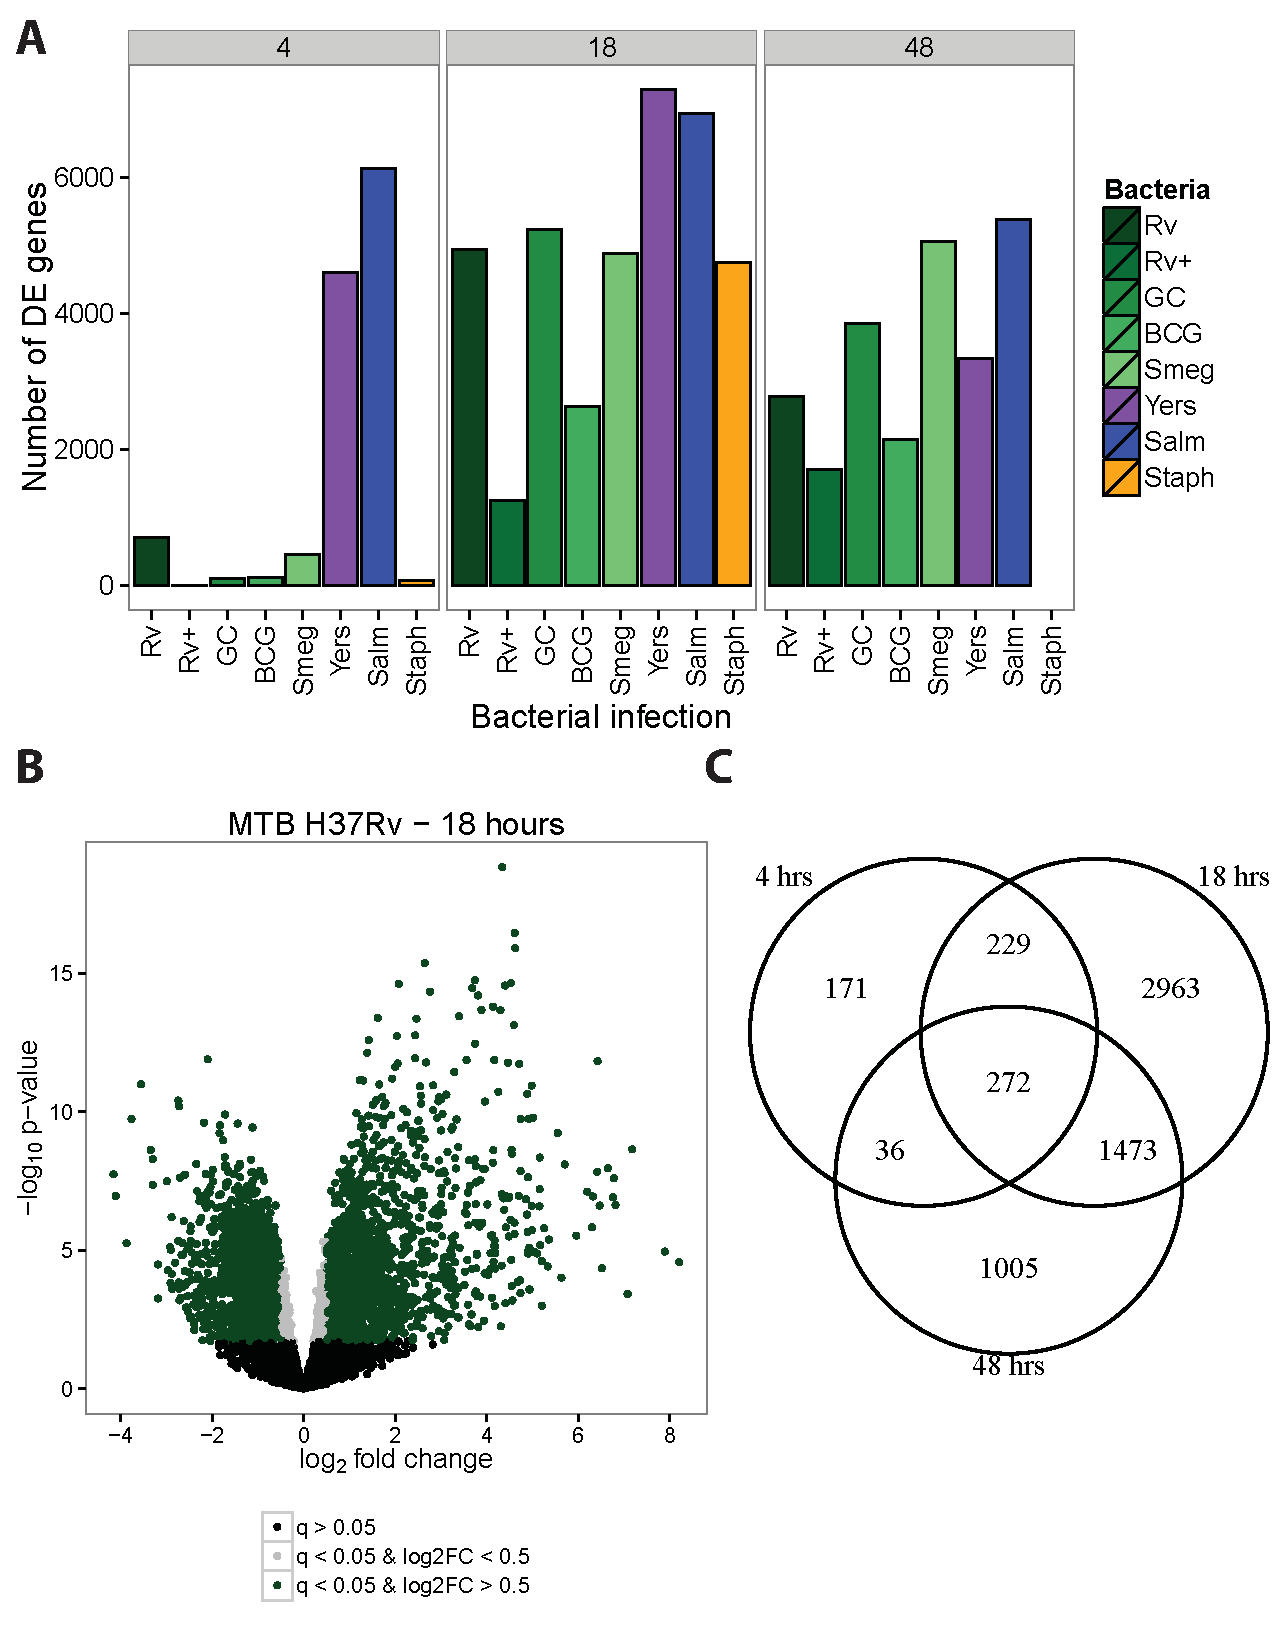
\includegraphics[width=5in]{img/ch02/fig-01-differential-expression.pdf}
\caption[Differential expression analysis.]{\textbf{Differential
    expression analysis.} We tested for differentially expressed genes
  for each bacterial infection by comparing it to its time-matched
  control. (A) We classified genes with q-value \textless{} 5\% as
  differentially expressed. The mycobacteria are labeled in shades of
  green. (B) As expected, there were large transcriptional changes 18
  hours post-infection with MTB H37Rv. Genes with q-value \textless{}
  5\% and absolute log\textsubscript{2} fold change greater than 0.5
  are labeled green, those with q-value \textless{} 5\% and absolute
  log 2 fold change less than 0.5 are labeled grey, and
  non-differentially expressed genes are labeled black. (C) The
  overlap in differentially expressed genes identified at 4, 18, and
  48 hours post-infection with MTB H37Rv.  }
\label{fig:differential-expression}
\end{figure}


\subsection{Joint analysis identifies bacteria-specific response
genes}\label{joint-analysis-identifies-bacteria-specific-response-genes}

In order to learn about variation in the innate immune response to
bacterial infection, we identified genes whose regulation was altered by
treatment with specific bacteria at specific timepoints. We first used a
naïve approach whereby we determined all the pairwise overlaps between
lists of DE genes across treatments (Supplementary Table \ref{tab:s7}). The caveat
of this strategy is that incomplete power can result in overestimating
the difference between treatments. In order to account for incomplete
power to detect DE genes when performing multiple pairwise comparisons,
we performed a joint Bayesian analysis, which we implemented using the
R/Bioconductor package Cormotif \citep{Wei2015} (see Methods for more
details). Using this approach, we classified genes into regulatory
patterns based on their expression levels following each of the
bacterial infections.

First, we examined the data across all the bacteria-time combinations.
Initially we built a model that classified genes into one of 14 separate
patterns based on their expression levels after each infection relative
to their expression level in the non-infected control (Supplementary
Fig. \ref{fig:joint-all-k14}). However, we found that a model with only six expression
patterns (Fig. \ref{fig:joint-all}; Supplementary Tables \ref{tab:s3},\ref{tab:s4}), where a subset of the
original 14 patterns are combined, is more intuitive from a biological
perspective; thus we proceeded with the reduced model. Broadly speaking,
we classified genes as responding in the early, middle, or late stages
of infection, and we characterized the response as temporary or
sustained. Pattern ``non-DE'' includes 4,245 genes whose expression
levels were unchanged in all the experiments. Pattern ``Yers-Salm''
includes 1,414 early response genes whose expression levels changed at
four hours post-infection with either \emph{Y. pseudotuberculosis} or
\emph{S. typhimurium}, but not after infection with other bacteria. The
genes in this pattern are enriched for gene ontology (GO) annotations
related to type I interferon signaling (e.g. \emph{SP100}, \emph{IFI35},
\emph{STAT2}), antigen presentation (\emph{HLA-A}, \emph{PSME1},
\emph{CTSS}), and apoptosis (\emph{CASP8}, \emph{TRADD}, \emph{FADD})
(Supplementary Table \ref{tab:s5}). Pattern ``18 h'' includes 3,201 middle
response genes whose expression levels changed exclusively at 18 hours
post-infection in response to all bacteria and is enriched for GO
annotations related to apoptosis (e.g. \emph{E2F1}, \emph{TP53},
\emph{WWOX}). Pattern ``48 h'' includes 1,204 late response genes whose
expression levels changed at 48 hours and is enriched for GO annotations
related to phagocytosis (e.g. \emph{MFGE8}, \emph{COLEC12}) and tumor
necrosis factor-mediated signaling (e.g. \emph{STAT1}, \emph{TRAF2},
\emph{TNFRSF14}). Pattern ``18 \& 48 h'' includes 1,926 middle-sustained
response genes whose expression levels changed at 18 and 48 hours and is
enriched for GO annotations related to the regulation of phagocytosis
(e.g. \emph{CD36}) and TLR signaling (\emph{TLR1}, \emph{TLR2},
\emph{MYD88}). Lastly, pattern ``All'' includes 738 early-sustained
genes whose expression levels changed after infection with all the
bacteria across all three timepoints and is enriched for GO annotations
related to type I interferon signaling (e.g. \emph{IRF1}, \emph{SOCS1},
\emph{IFIT3}), cytokine secretion (\emph{TNF}, \emph{IL10},
\emph{LILRB1}), and apoptosis (e.g. \emph{IRF7}, \emph{BCL2A1},
\emph{MCL1}).

\begin{figure}
\centering
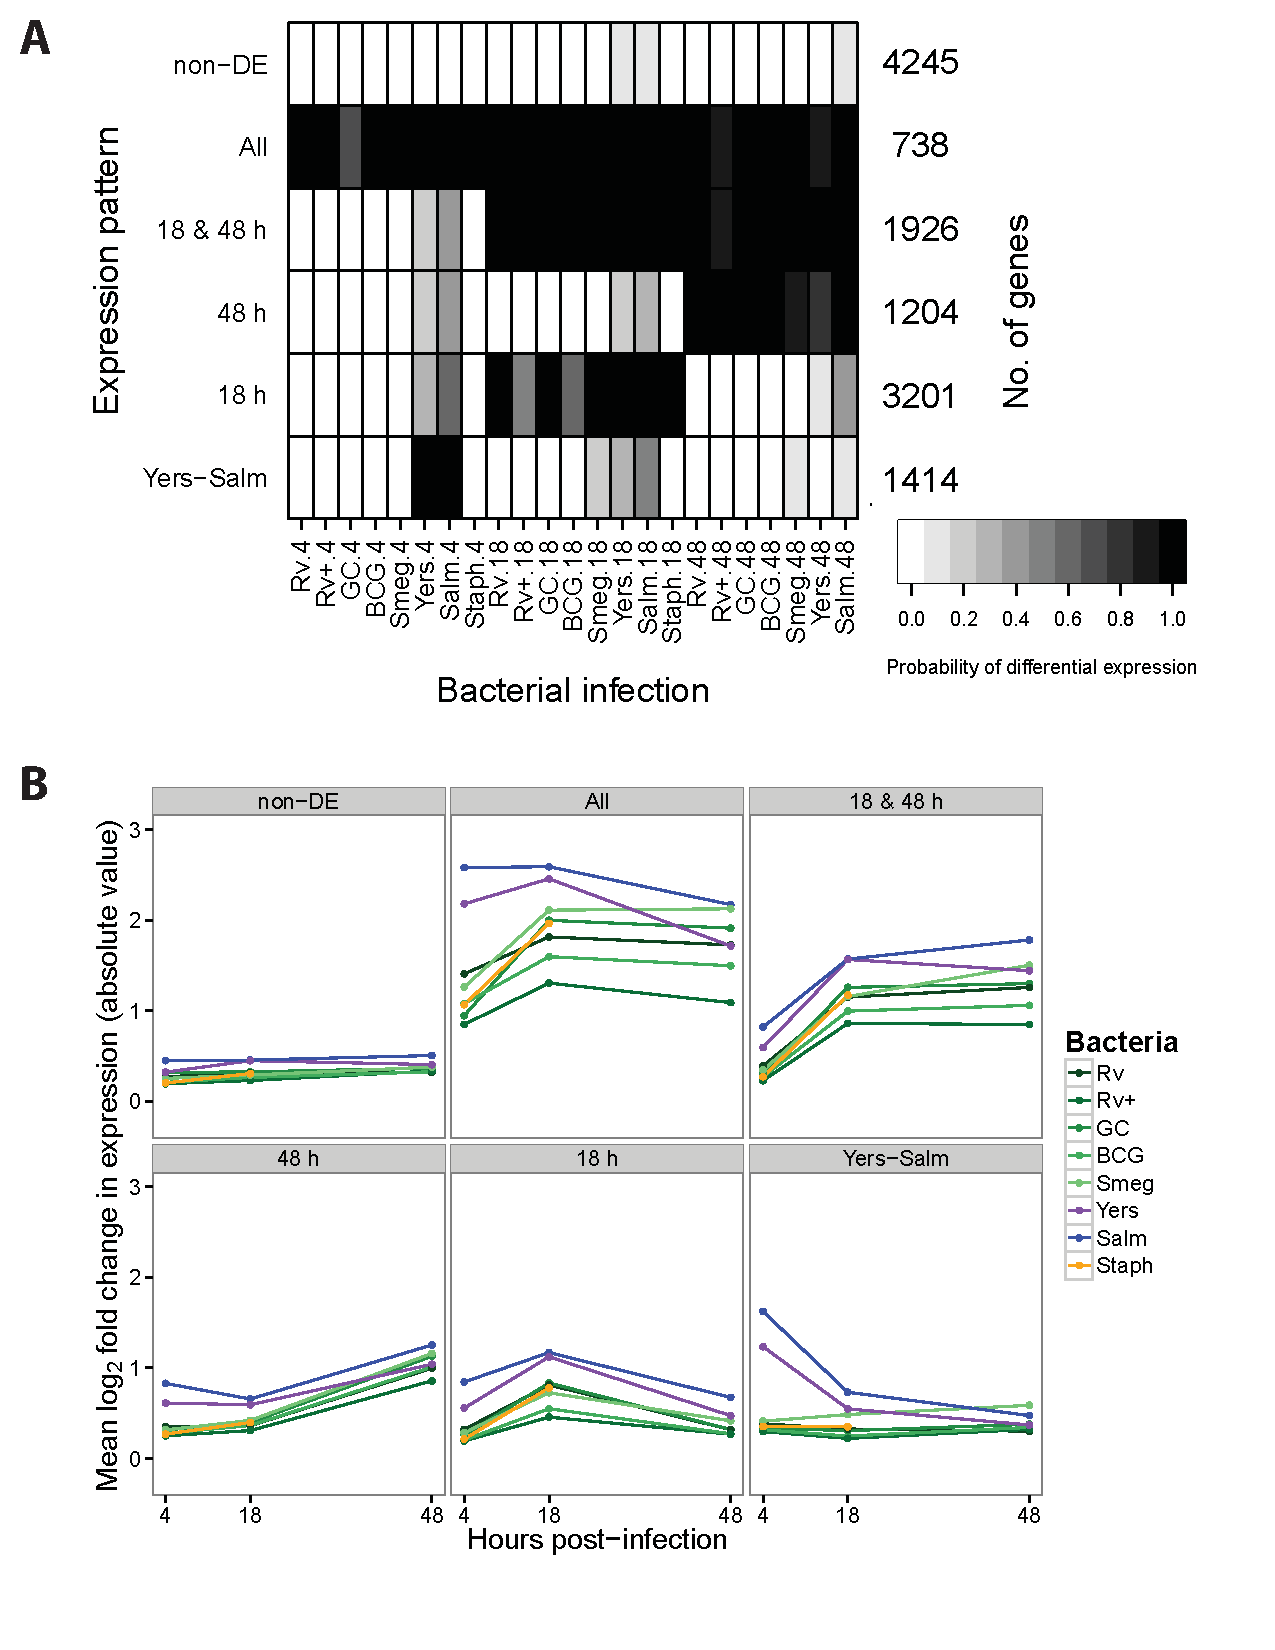
\includegraphics[width=5in]{img/ch02/fig-02-joint-all.pdf}
\caption[Joint Bayesian analysis.]{\textbf{Joint Bayesian analysis.}
  (A) Joint analysis of gene expression data from all three timepoints
  with Cormotif \citep{Wei2015} identified six expression patterns:
  ``non-DE'', ``Yers-Salm'', ``18 h'', ``48 h'', ``18 \& 48 h'', and
  ``All''. The shading of each box represents the posterior
  probability that a gene assigned to the expression pattern (row) is
  differentially expressed in response to infection with a particular
  bacteria (column), with black representing a high posterior
  probability and white a low posterior probability. (B) Each data
  point is the mean log\textsubscript{2} fold change in expression
  (absolute value) in response to infection with the given bacteria
  for all the genes assigned to the particular expression pattern.}
\label{fig:joint-all}
\end{figure}

Next, we tested for more specific patterns by performing Cormotif
separately on the data from the middle (18 h) and late (48 h) stages of
infection. At 18 hours post-infection, we identified five separate
expression patterns (Fig. \ref{fig:joint-18h}; Supplementary Tables \ref{tab:s3},\ref{tab:s4}). Pattern
``non-DE'' includes 5,268 genes whose expression levels were unchanged
across all infections. Pattern ``All'' includes 4,424 genes whose
expression levels were affected by all infections (e.g. \emph{IL24},
\emph{IRF2}, \emph{TLR2}). Pattern ``MTB'' includes 177 genes whose
expression levels changed specifically in response to infection with
mycobacteria (e.g. \emph{NCF2}, \emph{TNFSF13}, \emph{CSF1}). These
genes had a high posterior probability of being DE 18 hours after
infection with MTB H37Rv, heat-killed H37Rv, MTB GC1237, and BCG.
Furthermore, the gray shading for \emph{M. Smegmatis} (Fig. \ref{fig:joint-18h}A)
signified an intermediate posterior probability for DE. In essence, this
pattern is a merger of two sets of genes that were not large enough to
be separated: one set that was DE across all five mycobacteria and
another that was only DE after infection with the MTB strains and the
closely-related BCG, but not \emph{M. Smegmatis}. Pattern ``Virulent'',
in contrast, includes 1,165 genes whose expression levels were less
strongly changed after infection with heat-inactivated MTB H37Rv or the
attenuated vaccine strain BCG compared to the other bacteria (e.g.
\emph{IL1R1}, \emph{IRF1}, \emph{PILRB}). Also the genes in this
category only have an intermediate probability of responding to the
non-pathogenic \emph{M. smegmatis}. Lastly, pattern ``Yers-Salm''
includes 1,694 genes whose expression levels changed preferentially
after infection with \emph{Y. pseudotuberculosis} or \emph{S.
typhimurium} (e.g. \emph{TLR8}, \emph{TGFB1}, \emph{IL18}).

\begin{figure}
\centering
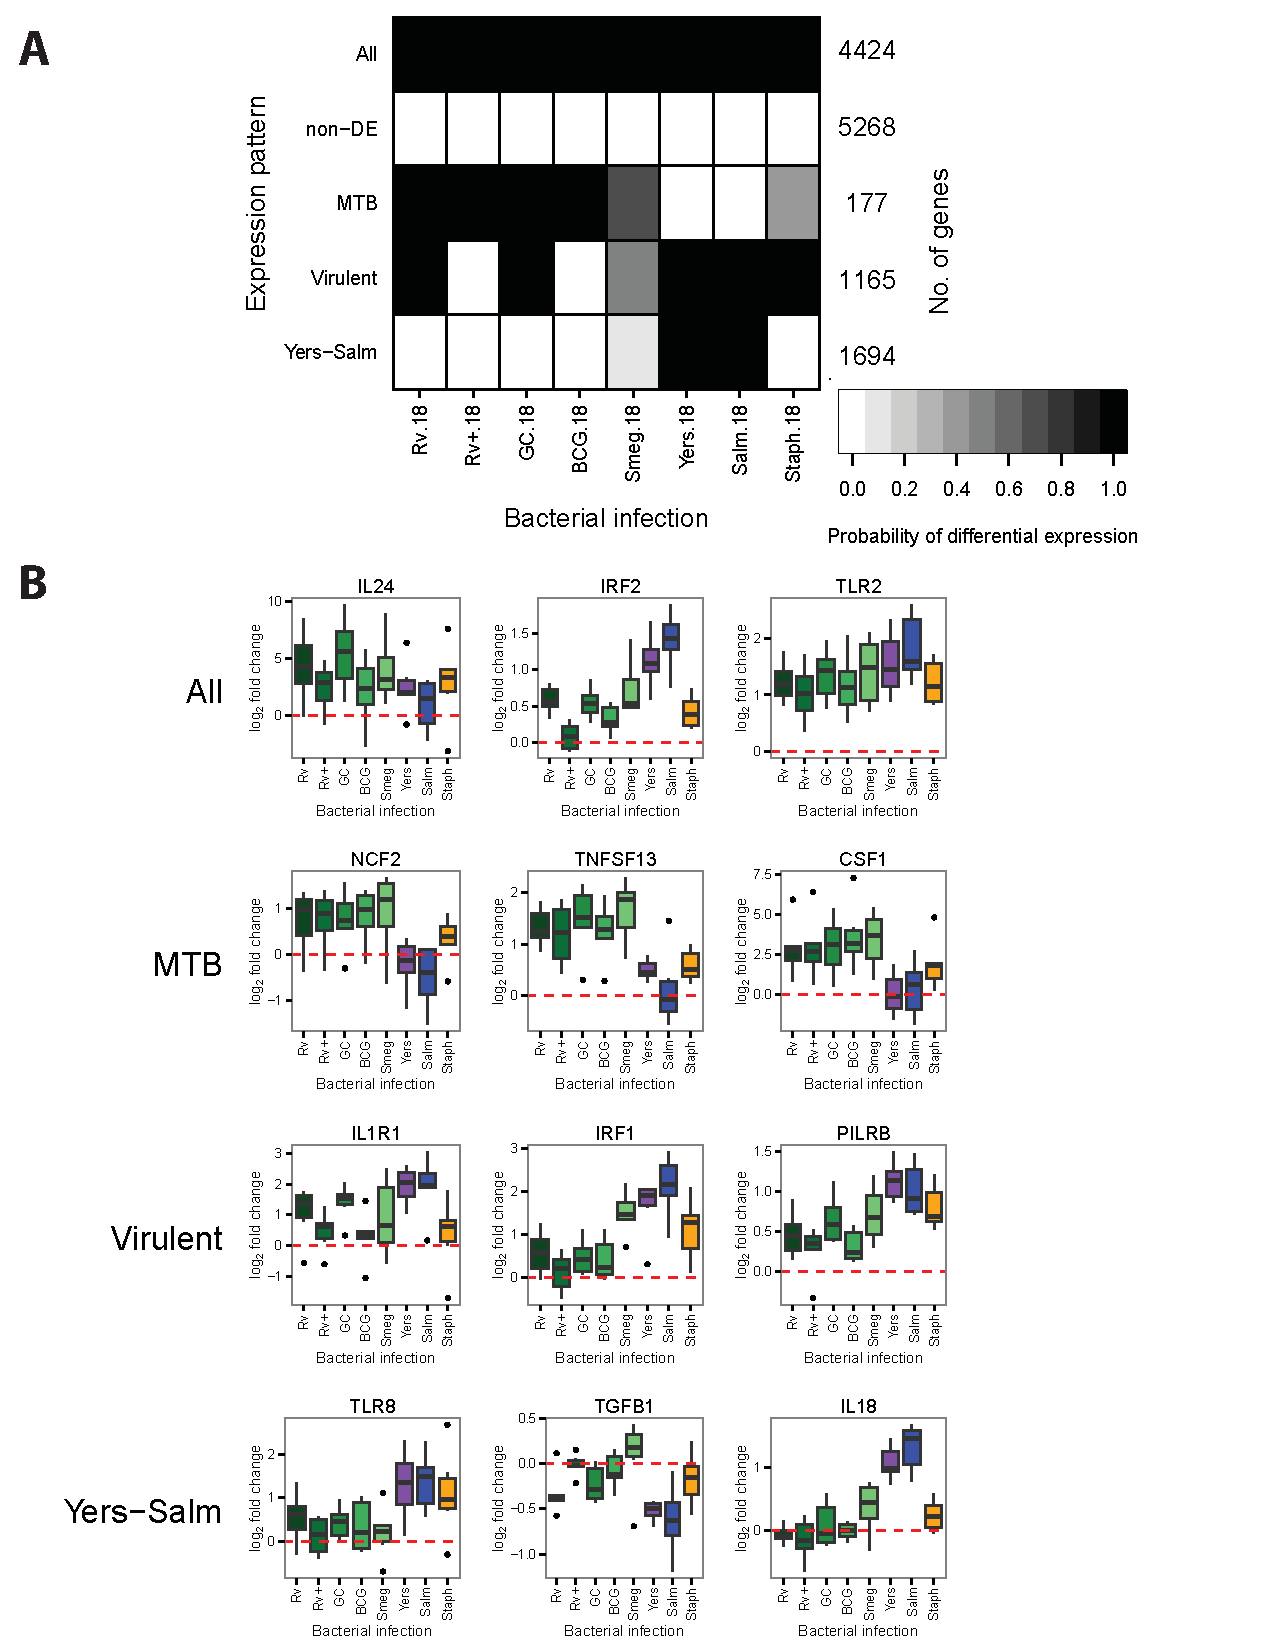
\includegraphics[width=5in]{img/ch02/fig-03-joint-18h.pdf}
\caption[Joint Bayesian analysis - 18 hours
  post-infection.]{\textbf{Joint Bayesian analysis - 18 hours
    post-infection.} (A) Joint analysis of gene expression data from
  18 hours post-infection with Cormotif identified five expression
  patterns: ``Yers-Salm'', ``Virulent'', ``MTB'', ``non-DE'', and
  ``All''. (B) Example genes from the different expression patterns.}
\label{fig:joint-18h}
\end{figure}

At 48 hours post-infection, we also discovered five expression patterns
(Fig. \ref{fig:joint-48h}; Supplementary Tables \ref{tab:s3},\ref{tab:s4}). While many of the patterns have
similar specificities to those observed at 18 hours post-infection,
there is only little overlap across timepoints with respect to the genes
comprising the patterns. For example, pattern ``Yers-Salm'' at 48 hours
includes 1,582 genes whose expression levels changed strongly after
infection with \emph{Y. pseudotuberculosis} or \emph{S. typhimurium}
(e.g. \emph{HLA-DPB1}, \emph{IL10RB}, \emph{CD248}), but only 263 of
these genes are also in the corresponding pattern when we considered the
data from the 18 hour timepoint. Similarly, at the 48 hour timepoint,
pattern ``MTB'' includes 288 genes whose expression levels changed
preferentially after infection with mycobacteria (e.g. \emph{CCL1},
\emph{ATP6V1A}, \emph{IL27RA}), but only 33 of these genes are in the
corresponding pattern at the 18 hour timepoint. Pattern ``Virulent''
includes 14 genes whose expression levels were not changed after
infection with heat-inactivated MTB H37Rv or the attenuated vaccine
strain BCG (e.g. \emph{MAP3K4}, \emph{SEMA4G}, \emph{BTG1}), and only
one of these also belongs to the pattern ``Virulent'' at 18 hours
post-infection.

\begin{figure}
\centering
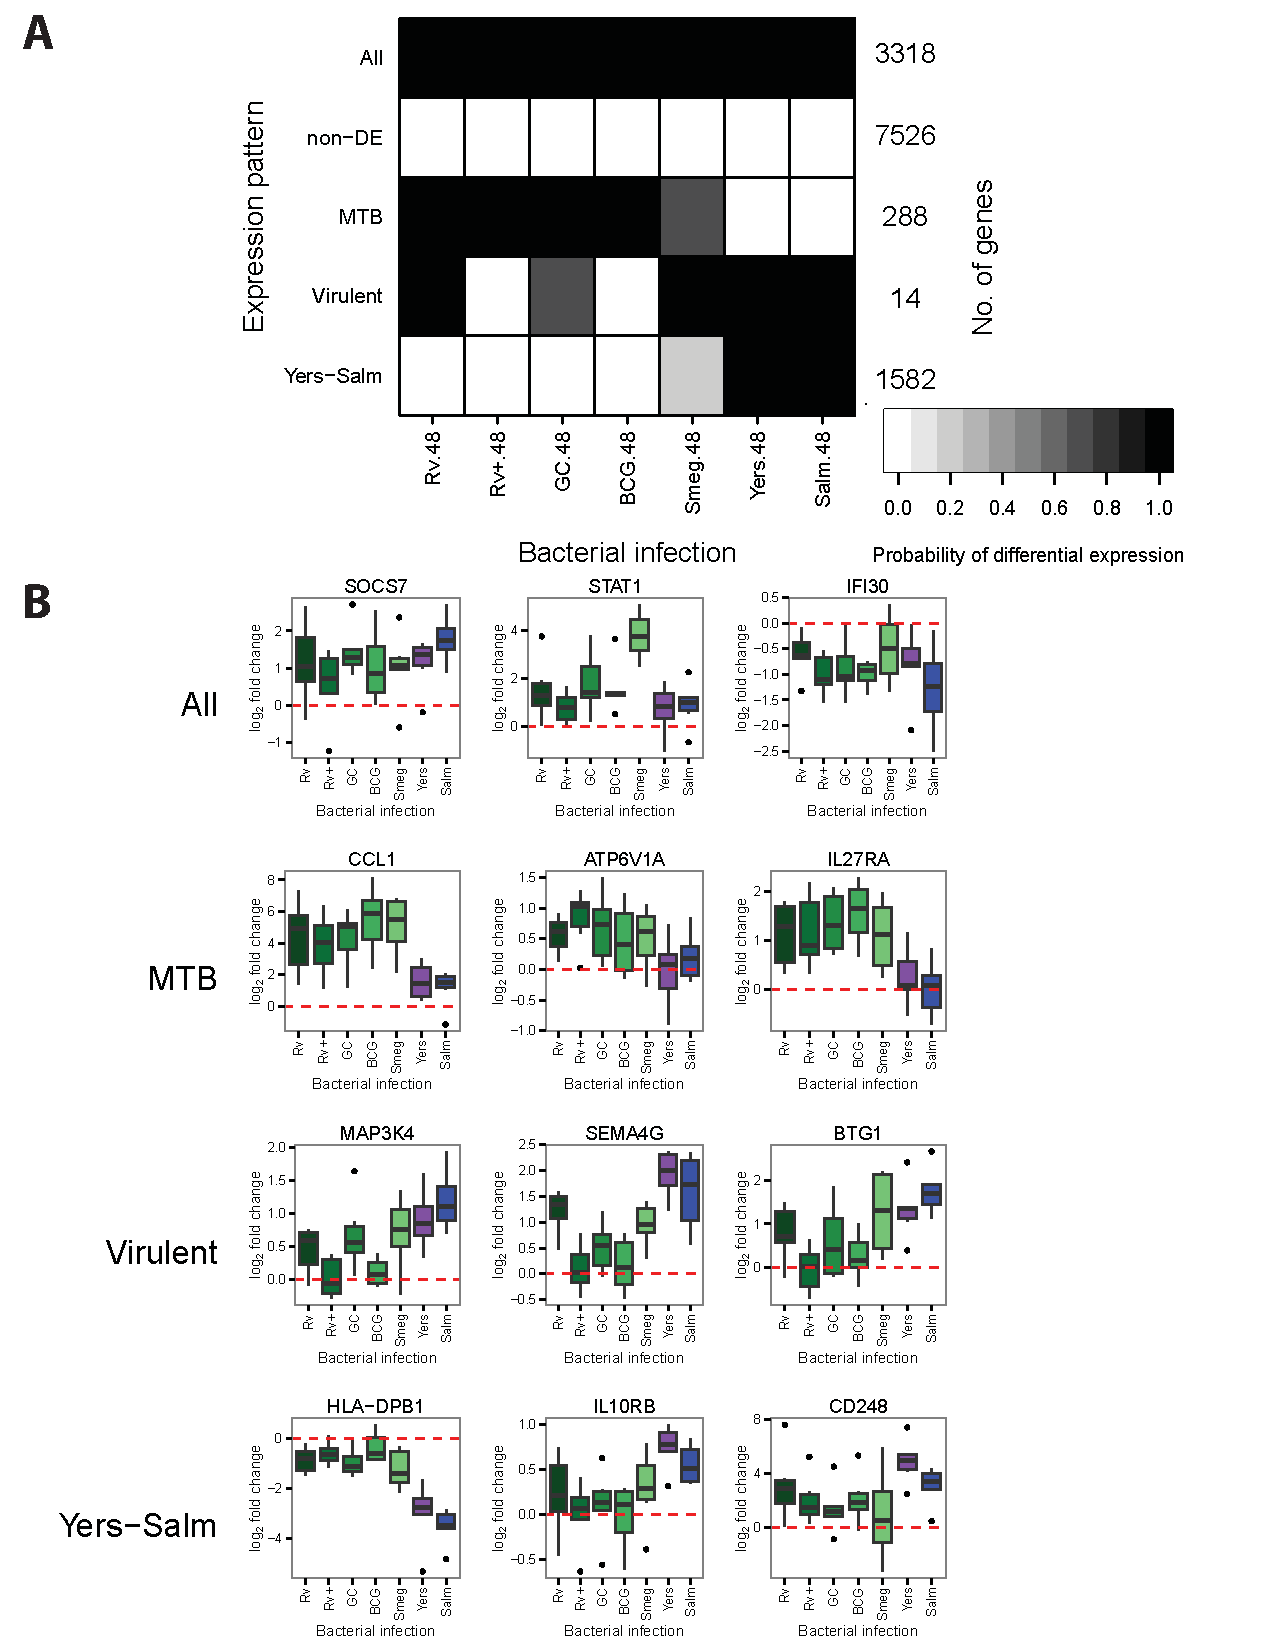
\includegraphics[width=5in]{img/ch02/fig-04-joint-48h.pdf}
\caption[Joint Bayesian analysis - 48 hours
  post-infection.]{\textbf{Joint Bayesian analysis - 48 hours
    post-infection.} (A) Joint analysis of gene expression data from
  48 hours post-infection with Cormotif identified five expression
  patterns: ``Yers-Salm'', ``Virulent'', ``MTB'', ``non-DE'', and
  ``All''. (B) Example genes from the different expression patterns.}
\label{fig:joint-48h}
\end{figure}

\subsection{Infection-induced response eQTLs are shared across
bacterial
infections}\label{infection-induced-response-eqtls-are-shared-across-bacterial-infections}

Using the gene expression patterns we identified by applying the joint
analysis approach, we investigated the specificity of previously
identified response eQTLs to infection with MTB H37Rv
\citep{Barreiro2012}. Since the response eQTLs were identified at 18
hours post-infection, we investigated the distribution of genes
associated with response eQTLs among the five patterns we found at that
timepoint (Figure 5A). Only one gene associated with a response eQTL was
also DE specifically in response to MTB (\emph{CMAS}). Otherwise, most
of the response eQTL-associated genes were classified as either DE
following infection with all bacteria or not DE in any infection. That a
large proportion of the genes associated with response eQTLs were not DE
in any of these experiments is likely due to the fact that the eQTL
study was performed in dendritic cells whereas our data were collected
from macrophages. Overall, our observations suggest that most of the
previously identified response eQTLs are genetic variants that affect
the human innate immune response to bacterial infection in general, and
not specifically the response to MTB H37Rv.

To provide further broad support for the interpretation that the
response eQTL genes are important for the innate response to bacterial
nfection in general, we considered the log\textsubscript{2} fold change
in expression values following infection (Fig. \ref{fig:differential-expression}). For each gene, we
calculated the mean log\textsubscript{2} fold change in expression level
across the eight bacterial infections at the 18 hour timepoint. Next, we
compared the absolute values of the log\textsubscript{2} fold change in
expression between genes associated with response eQTLs, genes
associated with general eQTLs (i.e.~genes associated with an eQTL pre-
and post-infection), and genes not found to be associated with an eQTL.
Since there was a large difference in the number of genes in these three
classes, we subsampled genes from each and calculated the mean of the
absolute values (and repeated this process 1000 times). We found that
the expression level of genes associated with response eQTLs is altered
to a larger degree (significantly higher effect size; \emph{P}
\textless{} 2.2 x e\textsuperscript{-16}; Figure 5B) following infection
compared to the genes in the other two classes.

\begin{figure}
\centering
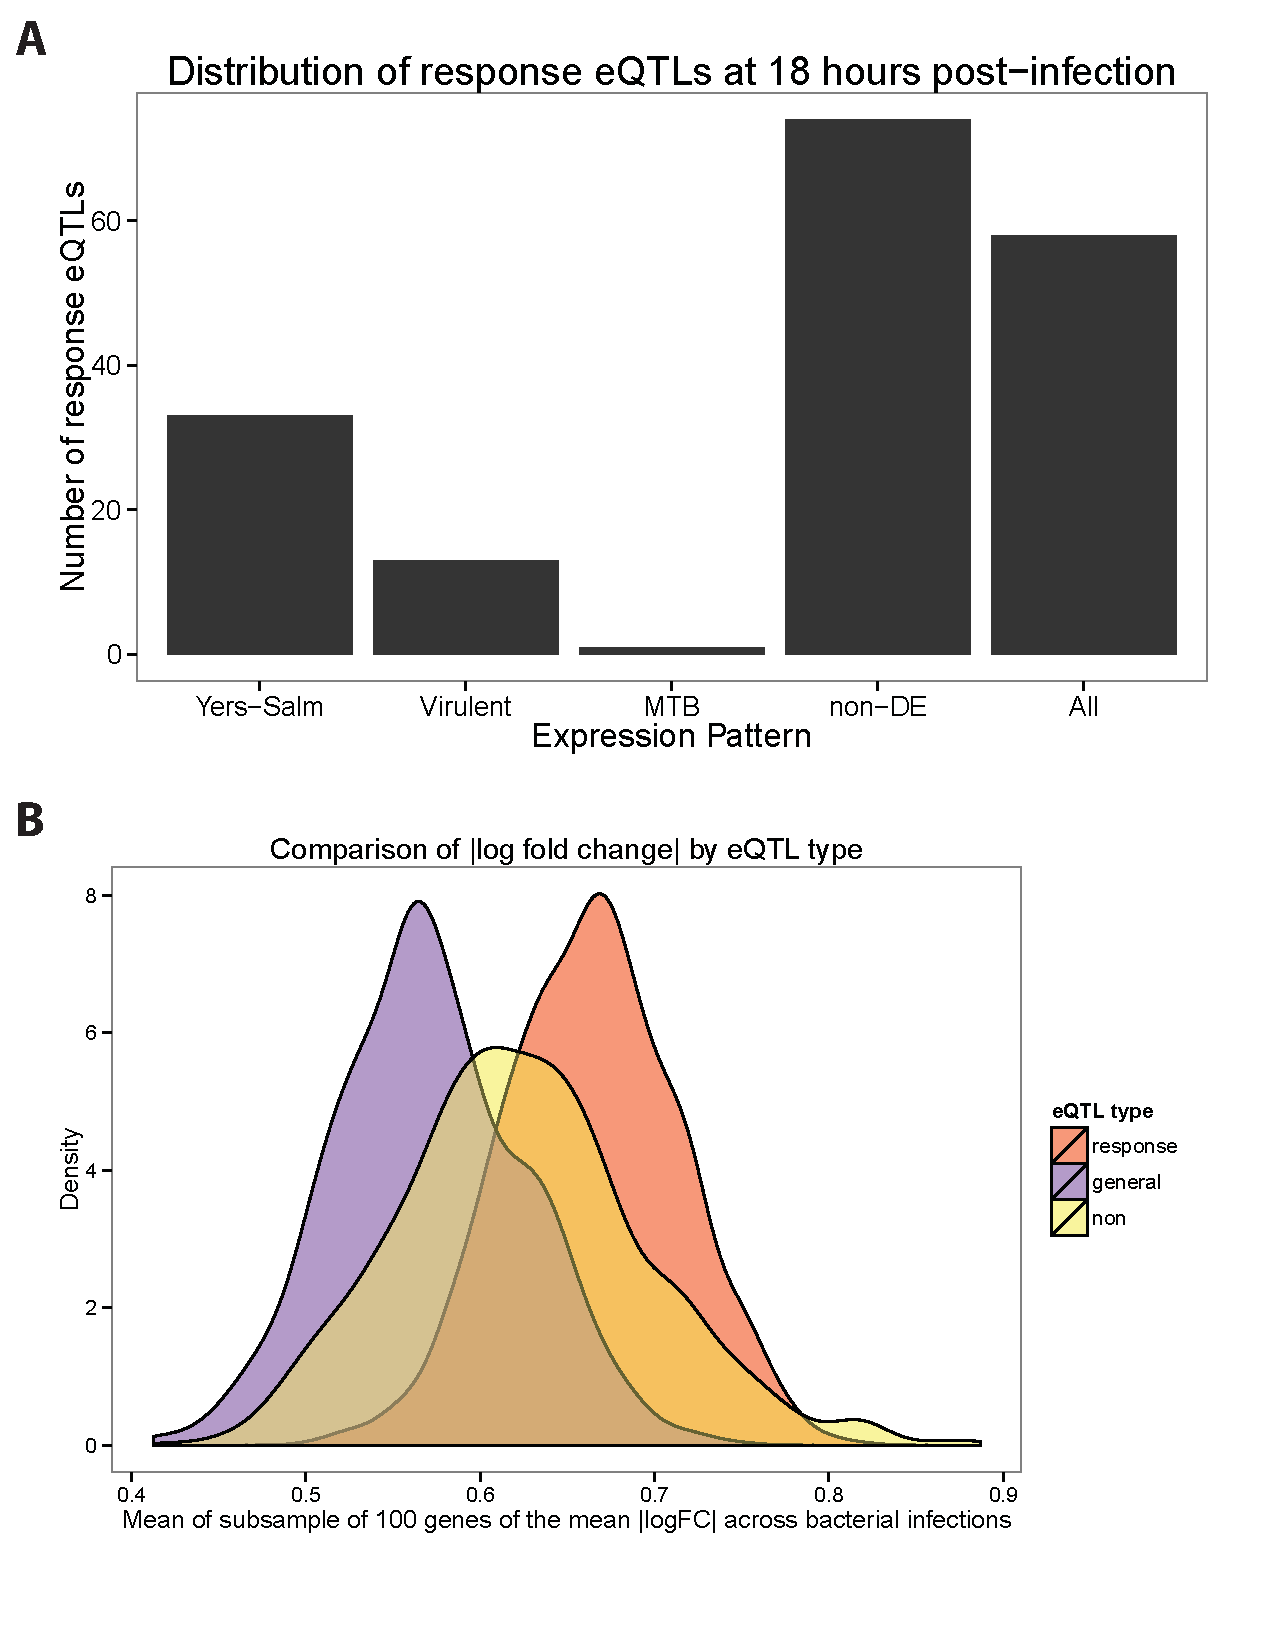
\includegraphics[width=5in]{img/ch02/fig-05-response-eqtl.pdf}
\caption[Response eQTLs at 18 hours post-infection.]{\textbf{Response
    eQTLs at 18 hours post-infection.} (A) We counted the number of
  response eQTLs from Barreiro et al. \citep{Barreiro2012} (179 out of
  the 198 were also expressed in our study) in each of the five gene
  expression patterns at 18 hours post-infection
  (Fig. \ref{fig:joint-18h}).  (B) We compared the mean
  log\textsubscript{2} fold change in expression across the 8
  bacterial infections at the 18 hour timepoint for three classes of
  genes: response eQTL genes (red), general eQTL genes (purple), and
  non-eQTL genes (yellow) (see Methods for details).  }
\label{fig:response-eqtl}
\end{figure}

\section{Discussion}\label{discussion}

\subsection{Bayesian analysis identified mycobacteria-specific
response
genes}\label{bayesian-analysis-identified-mycobacteria-specific-response-genes}

In order to identify general and treatment-specific gene regulatory
responses, we performed a joint Bayesian analysis of the data using
Cormotif \citep{Wei2015}. By jointly analyzing the data, as opposed to
comparing overlaps between independent lists of differentially expressed
genes generated using an arbitrary cutoff, we minimized the
identification of specific responses due to false negatives (i.e.~genes
that appear to be differentially expressed in response to a subset of
bacterial infections when in reality the response is similar across all
the infections). Similar to previous observations \citep{Huang2001,
Boldrick2002}, we found a large core transcriptional response to
infection. However, we also identified a novel subset of genes whose
regulation is preferentially altered in response to infection with
mycobacteria but not to the other bacteria we tested. Since these
responses are unique to infection with mycobacteria (at least in the
context of our study design), they may be promising candidates for
future studies that focus on the mechanisms by which mycobacteria
successfully subvert the human innate immune response. Since this study
does not extend to investigation of mechanisms, we do not have empirical
data with which to prioritize such possible candidate genes. Yet, the
reported functions of many of these genes often suggest mechanisms that
are relevant, and often quite specific, to MTB infection. Prioritizing
candidate genes in this way is not statistically valid, and one can
argue (and indeed, this has been shown \citep{Pavlidis2012}) that any
list of genes can be scrutinized to yield ``interesting relevant
stories''. We therefore offer these details in the context of a
discussion (rather than ``results''), to provide one set of alternative
explanations for our findings, and generate ideas for further
investigations.

For example, when we focused on the mycobacteria-specific regulatory
response 18 hours post-infection, we noticed an intriguing number of
genes that are involved in phagosome maturation (Supplementary Fig. \ref{fig:phago}). Broadly speaking, phagocytosed bacteria are killed by vesicular
proton pumps, which lower the pH inside the phagosome, and lysosomal
fusion. This process occurs once a phagosome has matured through a
series of steps mediated by the exchange of Rab GTPases \citep{Vergne2004,
Mortellaro2009}. A unique property of mycobacteria is their ability
to survive inside the macrophage by inhibiting phagosome maturation
\citep{Hestvik2005}. As part of this strategy, the bacterium recruits
\emph{RAB22A} to MTB-containing phagosomes \citep{Roberts2006}. Indeed,
we found the \emph{RAB22A} gene to be upregulated in response to
infection with mycobacteria (Supplementary Table \ref{tab:s4}). Similar GTPases
whose regulation was altered following mycobacterial infections include
\emph{RAP2A} (upregulated), \emph{RAB3A} and \emph{RAB33A} (both
downregulated). In addition, the vesicular (v)-ATPase subunit
\emph{ATP6V1D} was exclusively upregulated in response to mycobacterial
infection. Thus, the mycobacteria-specific response we identified
includes genes putatively involved in mycobacteria-specific survival
mechanisms.

An additional intriguing example involves the \emph{NCF2} gene. This is
a potential candidate gene whose expression level was affected
specifically by infection with mycobacteria at 18 hours post-infection.
Neutrophil cytosolic factor 2 (\emph{NCF2}, also known as
\emph{p67phox}) is a subunit of the phagocyte NAPDH oxidase, which is
responsible for generating reactive oxygen species used to fight
intracellular pathogens \citep{Ehrt2001, Myers2003, Babior2004,
Bustamante2011, Kim2011c, Deffert2014}. These reactive oxygen
species may also serve a signaling role in activating other immune cell
types to ensure proper granuloma formation and killing of mycobacteria
\citep{Deffert2014a}. Loss-of-function mutations in subunits of the NAPDH
oxidase cause chronic granulomatous disease (CGD) \citep{Deffert2014},
which is characterized by the formation of granulomas throughout the
body due to the inability of phagocytes to kill the ingested pathogens.
In contrast to wild type animals, mice with mutations in subunits of the
phagocyte NAPDH oxidase develop tuberculosis after infection with the
vaccine strain, BCG \citep{Deffert2014a}. Humans who are administered the
vaccine before being diagnosed with CGD also develop the disease
\citep{Deffert2014}.

At 48 hours post-infection (Fig. \ref{fig:joint-48h}), the mycobacteria-specific
response was enriched with genes annotated (based on GO) as having a
role in ``response to vitamin D'' (Supplementary Table \ref{tab:s5}; Supplementary
Figure \ref{fig:vitD}). Individuals with low circulating levels of vitamin D are
more susceptible to developing tuberculosis \citep{Zodpey2007,
Nnoaham2008}, and vitamin D has been investigated as a supplemental
therapy for the treatment of tuberculosis, though with mixed results
\citep{Martineau2007, Lucas2014, Xia2014, Kearns2015}. Vitamin D has
been found to be important for innate immune cells to fight MTB
\citep{Liu2006, Verway2013, Xu2014}; however, it is also an important
pathway for generic bactericidal activity \citep{Hewison2011}. Consistent
with its role in the innate immune response, both the enzyme that
converts vitamin D to its active form (\emph{CYP27B1}) and its receptor
(\emph{VDR}) are upregulated in response to any of the infections
(pattern ``All''; Fig. \ref{fig:joint-48h}). Yet, the regulation of other genes involved
in the response to vitamin D was only affected by infection with MTB.
\emph{PIM1}, a serine/threonine kinase that binds the VDR and enhances
transcription of its target genes \citep{Maier2012}, is upregulated in
response to the mycobacteria (pattern ``MTB'', Fig. \ref{fig:joint-48h}). Interestingly,
the increased expression level of \emph{PIM1} in T-cells was
successfully used in a six-gene classifier of patients with active
versus latent TB infections \citep{Jacobsen2011}. Another gene, the
chemokine \emph{CXCL10} (also known as interferon gamma-induced protein
10 or IP-10), is also upregulated in response to mycobacterial infection
(pattern ``MTB'', Fig. \ref{fig:joint-48h}). Discordant with the observed increase in
expression of \emph{CYP27B1}, \emph{VDR}, and \emph{PIM1} in response to
infection, treatment with vitamin D usually leads to the reduction of
\emph{CXCL10} expression and secretion in multiple cell types
\citep{Gysemans2005, Adorini2005, Scolletta2013}. In fact,
supplementation with vitamin D decreased serum levels of CXCL10 in TB
patients \citep{Coussens2012}. This suggests that the immunosuppresive
effect of vitamin D signaling is insufficient to overcome the
pro-inflammatory response to mycobacterial infection. This observation
is in concordance with past studies which found increased expression of
\emph{CXCL10}, as well as increased secretion level from macrophages,
following infection with MTB \citep{Zhu2006, Verway2013}. Interestingly,
a polymorphism in \emph{CXCL10} was found to be associated with
susceptibility to tuberculosis in a Chinese population \citep{Tang2009,
Azad2012}. Overall, these observations provide support for the
importance of vitamin D signaling for specifically fighting
mycobacterial infections.

Another gene of interest from the mycobacteria-specific expression
pattern at 48 hours post-infection is chemokine (C-C motif) ligand 1
(\emph{CCL1}), which stimulates migration of human monocytes
\citep{Miller1992} (Fig. \ref{fig:joint-48h}B). Thuong et al. identified \emph{CCL1} as
being induced to a greater extent in MTB-infected macrophages (4 hours
post-infection) isolated from individuals with pulmonary TB compared to
macrophages from individuals with latent TB infections
\citep{Thuong2008}. Put together, our observations and those of Thuong
and colleagues suggest that \emph{CCL1} is involved in the pathogenesis
of TB. Further supporting this notion, Thuong et al. also found a
genetic association between variants in the \emph{CCL1} region and TB
susceptibility \citep{Thuong2008}. However to date, subsequent genetic
association studies investigating \emph{CCL1} have reported mixed
results \citep{Tang2011, Ozdemir2013}.

One caveat of the joint Bayesian analysis is that we were not able to
classify genes into unusual patterns (because this approach can only
discover expression patterns shared by a large number of genes and, by
definition, only few genes fall into ``unusual'' patterns). For example,
unusual patterns of interest include changes in expression specifically
in response to some but not all of the mycobacterial infections. One
gene that satisfied this pattern is the dual specificity phosphatase 14
(\emph{DUSP14}). We specifically examined the expression data for this
gene because it was previously associated with an MTB infection response
eQTL in dendritic cells \citep{Barreiro2012}, and consequently when the
eQTL results were used as a prior - \emph{DUSP14} was found to be
significantly associated with TB susceptibility. Moreover, knocking down
\emph{DUSP14} expression via siRNA in murine macrophages resulted in a
lower bacterial load 90 hours post-infection with MTB H37Rv
\citep{Jayaswal2010}. In our joint Bayesian analysis, \emph{DUSP14} was
not classified as one of the genes whose regulation was altered in
response to infection with mycobacteria. Yet, \emph{DUSP14} was
upregulated at 18 hours post-infection with MTB H37Rv (q-value: 16\%),
MTB GC1237 (q-value: 3\%), and BCG (q-value: 9\%); and downregulated
post-infection with \emph{S. typhimurium} (q-value: 9\%) (Supplementary
Fig. \ref{fig:dusp14}). Thus, our data lends further support for the role of
\emph{DUSP14} as a TB susceptibility gene.

\subsection{Little evidence for strain-specific transcriptional
response to
infection}\label{little-evidence-for-strain-specific-transcriptional-response-to-infection}

There are six major families of MTB that differ in their geographic
distribution and virulence \citep{Gagneux2006, Comas2009}. Strains from
these families are known to differ in their growth rates inside
macrophages \citep{Li2002}, expression levels of bacterial genes
\citep{Homolka2010, Rose2013}, and cell wall lipid composition
\citep{Krishnan2011}. Previous studies have found that different MTB
strains induce different innate immune responses in human cell lines and
other infection models \citep{Coscolla2010}. A dominate narrative is that
MTB strains from East Asia, referred to as the Beijing family (Gagneux
et al. classified it as MTB lineage 2 \citep{Gagneux2006}), are more
virulent because they induce a lower proinflammatory immune response
compared to the common laboratory strains \citep{Manca2001, Manca2004,
Reed2004, Tanveer2009, Wang2010b}. However, other studies have
reported the opposite, namely that Beijing strains induce a larger
proinflammatory response \citep{Chacon-Salinas2005}, or a conflicting
response in which various pro- and anti-inflammatory cytokines are
differentially regulated \citep{Rocha-Ramirez2008, Koo2012} compared to
laboratory strains.

In our study, albeit with a small sample size, we found no marked
differences between the transcriptional response to infection with MTB
H37Rv or MTB GC1237, a Beijing strain (Supplementary Fig. \ref{fig:Rv-v-GC};
Supplementary Table \ref{tab:s8}). Furthermore, the pro-inflammatory cytokines
\emph{TNF} and \emph{IL6} and the anti-inflammatory cytokine \emph{IL10}
were strongly upregulated in response to both strains of MTB
(Supplementary Fig. \ref{fig:ex-cytokines}). This observation is in concordance with Wu et
al., who also reported no apparent difference in the transcriptional
response of THP-1 cells to infection with MTB H37Rv versus multiple
Beijing strains \citep{Wu2012}. Thus the increased virulence of the
Beijing family of MTB strains may be due to mechanisms not assayed in
this study such as post-transcriptional effects, cell-cell signaling,
and environmental stimuli. It should be noted, however, that not all
Beijing strains are equally virulent \citep{Dormans2004, Sinsimer2008}
and that MTB H37Rv is a laboratory-adapted strain that has evolved
independently in different laboratories \citep{Ioerger2010}.

\subsection{Differences in response to virulent versus attenuated
pathogens are not
mycobacteria-specific}\label{differences-in-response-to-virulent-versus-attenuated-pathogens-are-not-mycobacteria-specific}

To better understand the interaction between MTB and macrophages, we
included in our study both virulent mycobacteria (MTB strains H37Rv and
GC1237) and attenuated mycobacteria (heat-inactivated MTB H37Rv and the
vaccine strain BCG). Overall, the response to infection with either
virulent or attenuated mycobacteria was similar (Figures 3,4). This
observation was unsurprising because it has been previously demonstrated
that infections with inactivated pathogens (in fact, even individual
pathogen components) are able to largely recapitulate the
transcriptional response to infection \citep{Huang2001, Boldrick2002,
Nau2002, Jenner2005}. In other words, as expected, the
transcriptional response to infection is largely driven by the antigens
present.

Yet, the responses to inactivated pathogens or individual pathogen
components in past studies were not identical to the responses to live
pathogens, suggesting a potential role for bacterial manipulation of the
immune response. For example, it is known that BCG lacks the locus
containing the ESX-1 secretion system, which is critical for MTB
virulence \citep{Behr1999, Pym2002, Hsu2003, Simeone2009}. In our
study we also observed differences between the response to virulent and
attenuated mycobacteria. Specifically, there are 1,165 genes in the
expression pattern ``Virulent'' at 18 hours post-infection (Fig. \ref{fig:joint-18h})
and 14 genes that comprise of the ``Virulent'' pattern at 48 hours
post-infection (Fig. \ref{fig:joint-48h}). Importantly, these genes are also
differentially expressed in response to the other virulent infections in
our study, and thus they are not specifically due to the manipulations
of the host cell by virulent mycobacteria.

We attempted to identify a gene expression pattern that specifically
represented differences in virulence only in the mycobacteria, yet we
never saw such a pattern. It is important to note that had we simply
performed a simple pairwise analysis of the overlap of DE genes between
MTB and BCG infections, our results would be quite different
(Supplementary Table \ref{tab:s7}). Yet, a pairwise analysis is misleading in the
context of the entire study. Indeed, by accounting for incomplete power
by using the joint Bayesian model and including other bacterial species,
we avoided attributing many differentially expressed genes specifically
to the differences in the immune evasion mechanisms used by MTB and BCG.
We conclude that either a larger sample size or a different experimental
system is required to find specific differences between the response to
infection with MTB and BCG.

\subsection{Previously identified response eQTLs affect response to
bacterial infection in
general}\label{previously-identified-response-eqtls-affect-response-to-bacterial-infection-in-general}

In a previous study, we identified response eQTLs that were associated
with gene expression levels in MTB-infected human dendritic cells. We
investigated the expression pattern of genes associated with the
response eQTLs in our study. Using the five expression patterns
identified by the joint Bayesian analysis at 18 hours post-infection, we
examined the distribution of response eQTL genes and discovered that
these genes were not enriched in the mycobacteria-specific expression
pattern (Figure 5A). Instead, many were differentially expressed across
all the infections (pattern ``All''). Thus, response eQTLs modulate the
inter-individual response to infection with diverse types of bacteria.
That said, one gene was both associated with a response eQTL and
specifically differentially expressed following mycobacterial infection.
Though this result does not represent a significant enrichment of
response eQTL genes among those whose regulation was affected
specifically by infection with MTB, the identity of the gene renders the
observation intriguing. \emph{CMAS} (cytidine monophosphate
N-acetylneuraminic acid synthetase), is an enzyme that is involved in
the processing of sialic acid, which is then added to cell surface
glycoproteins and glycolipids. Glycoproteins are known to be important
in many functions of the immune response, including initial pathogen
detection (e.g.~TLRs) and antigen presentation (e.g.~major
histocompatibility complex (MHC) molecules) \citep{Wolfert2013,
Johnson2013, Crespo2013}. We suggest that this gene is an
interesting candidate for further understanding both MTB pathogenesis
and inter-individual susceptibility to tuberculosis.

\subsection{Conclusions}\label{conclusions}

By jointly considering data from multiple infection treatments, using a
variety of bacteria, we have classified distinct innate immune
transcriptional response patterns. The most inclusive pattern was a
response to all the bacterial infections, indicating that the receptors
that bind the diverse antigens present on the different bacteria
converge to largely similar signaling pathways. We also found an
expression response pattern specific to mycobacterial infections, the
main focus of the current study. At 18 hours post-infection, the
mycobacteria response pattern includes genes involved in phagosome
maturation and the NAPDH oxidase subunit \emph{NCF2}. At 48 hours
post-infection, it includes genes involved in the response to vitamin D
and the chemokine \emph{CCL1}. We found that the response to infection
with different MTB strains was highly similar. Furthermore, the
differences we identified between the response to MTB and the vaccine
strain BCG were not mycobacteria-specific, but likely represent a
difference between the innate immune response to virulent and
non-virulent (or attenuated) pathogens. Lastly, we identified a single
gene, \emph{CMAS}, which is both associated with a response eQTL to MTB
infection, and whose regulation is altered specifically when we infected
the cells with mycobacteria. This gene is thus an especially promising
candidate for future studies of TB susceptibility.

\section{Methods}\label{methods}

\subsection{Ethics Statement}\label{ethics-statement}

Buffy coats were obtained from healthy donors after informed consent.
The blood collection protocols were approved by both the French Ministry
of Research and a French Ethics Committee under the reference DC-2008-68
collection 2. The blood collection was carried out in accordance with
these approved protocols by the Etablissement Français du Sang.

\subsection{Sample collection and macrophage
differentiation}\label{sample-collection-and-macrophage-differentiation}

We collected buffy coats (\textasciitilde{}50 mL) from six healthy
donors. Next we isolated peripheral blood mononuclear cells (PBMCs) via
Ficoll-Paque centrifugation \citep{Rivero-Lezcano2012} and enriched for
monocytes via positive selection with beads containing CD14 antibodies
\citep{Barreiro2012}. Then we differentiated the monocytes into
macrophages by culturing for 6-7 days in RPMI buffer supplemented with
macrophage colony-stimulating factor (M-CSF) \citep{Tailleux2003}.

\subsection{Bacterial infection}\label{bacterial-infection}

For each bacterial infection (Table \ref{tab:bacteria}), we treated the macrophages with
a multiplicity of infection (MOI) of 2:1. After one hour, we washed the
macrophages five times with phosphate-buffered saline (PBS) and treated
them with gentamycin (50 $mu$g/$mu$L) to kill all extracellular bacteria.
After one hour of antibiotic treatment, we changed the medium to a lower
concentration of gentamycin (5 $mu$g/$mu$L), which marked the zero timepoint
of the study. We allowed the cells to grow for 4, 18, or 48 hours before
lysing them with QIAzol Lysis Reagent and then storing them at -80° C.
We chose these timepoints based on a previous analysis of the human
transcriptional response to infection with MTB \citep{Tailleux2008}. No
data is available for 48 hours post-infection with \emph{S.
epidermidis}. After escaping the macrophages upon cell death, sufficient
\emph{S. epidermidis} were able to proliferate in the
gentmycin-supplemented medium to contiminate the entire well by 48 hours
post-infection.

\subsection{RNA extraction, library preparation, and
sequencing}\label{rna-extraction-library-preparation-and-sequencing}

We extracted RNA using the QIAgen miRNeasy kit. There were a total of 13
batches of 12 samples each (6 individuals x 9 conditions x 3 timepoints,
minus 48 hours post-infection with \emph{S. epidermidis}). We designed
the batches to maximally partition the variables of interest
(individual, condition, timepoint) in order to minimize the introduction
of biases due to batch processing \citep{Auer2010}. To assess RNA
quality, we measured the RNA Integrity Number (RIN) with the Agilent
Bioanalyzer (Supplementary Table \ref{tab:s6}). Importantly, there were no
significant differences in the RIN (mean of 7.8 $\pm$ 2.0) between the
bacterial infections or between the timepoints (Supplementary Fig. \ref{fig:rin-and-reads}B). In batches of 12 samples, we added barcoded adapters (Illumina
TruSeq RNA Sample Preparation Kit v2) and sequenced 50 base pairs single
end over multiple flow cells on the Illumina HiSeq 2500.

\subsection{Mapping, counting, and
normalization}\label{mapping-counting-and-normalization}

We mapped the short reads to the human genome (hg19) using the Subread
algorithm \citep{Liao2013} and discarded those that mapped non-uniquely.
Next, we obtained the read counts for each Ensembl protein-coding gene
(biotype: ``protein\_coding'') with the featureCounts algorithm, which
sums the reads falling in the union of all exons of a gene and discards
reads mapping to more than one gene \citep{Liao2013a}. There were no
significant differences in the number of mapped exonic reads (mean of
41.8 $\pm$ 21.2 million per sample) between the bacterial infections or
between the timepoints (Supplementary Fig. \ref{fig:rin-and-reads}A). We removed genes with
fewer than one count per million exonic reads in fewer than six samples.
To account for differences in the read counts at the extremes of the
distribution, we normalized the samples using the weighted trimmed mean
of M-values algorithm (TMM) \citep{Robinson2010}.

\subsection{Differential expression
analysis}\label{differential-expression-analysis}

To assess the quality of the data, we performed principal components
analysis (PCA) of the TMM-normalized log\textsubscript{2}-transformed
counts per million (CPM). PC2 separated the samples by timepoint, but
PC1 was associated with the RIN score and the processing batch
(Supplementary Fig. \ref{fig:pca}A). After the effects of RIN score and
processing batch were removed with the function removeBatchEffect from
the limma package \citep{Ritchie2015}, PC1 separated the samples by
timepoint and PC2 separated the infected and control samples
(Supplementary Fig. \ref{fig:pca}B). We protected the variables of interest
(individual, bacteria, timepoint) when regressing the effects of RIN
score and processing batch by including them in the linear model used by
removeBatchEffect. However, the result was similar if they were not
protected since the variables of interest were partitioned across the
processing batches (Supplementary Fig. \ref{fig:pca}C). All figures displaying
expression data were generated using the batch-corrected data.

To confirm that the transcriptional response to MTB infection in our
study was consistent with previous observations, we compared our MTB
infected samples and their time-matched controls to the MTB infected
samples and zero timepoint control from Tailleux et al., 2008
\citep{Tailleux2008}. Despite differences in the technology used to assay
gene expression (RNA-seq versus microarray) and the method used to
isolate the macrophages (positive versus negative selection), we still
observed a common transcriptional signature of infection using PCA
(Supplementary Fig. \ref{fig:tailleux2008}).

For the standard analysis, we tested for differential expression using
limma+voom \citep{Smyth2004, Smyth2005, Law2014} because it has been
shown to perform well with sufficient sample size (n \textgreater{}= 3
per condition) \citep{Rapaport2013, Soneson2013}. Based on the PCA
results, we included RIN score and processing batch as covariates in the
model. We corrected for multiple testing with the Benjamini \& Hochberg
false discovery rate (FDR) \citep{Benjamini1995} and considered genes
with q-value less than 5\% to be differentially expressed.

Since we were interested in the shared and differential response to
infection with the different bacteria, we performed a joint Bayesian
analysis using the Cormotif algorithm \citep{Wei2015}. Cormotif shares
information across experiments, in this case infections, to identify the
main patterns of differential gene expression (which it refers to as
\emph{correlation motifs}) and assigns each gene to one of these gene
expression patterns. One caveat of the Cormotif algorithm is that is
does not distinguish the direction of the effect across infections. In
other words, a gene that is assigned to an expression pattern could be
differentially expressed in different directions across the infections.
However, in this data set, this was rarely observed (Supplementary Table
\ref{tab:s9}).

In practice, we had to make several modifications when using Cormotif.
First, since the method was developed for microarray data, we used the
batch-corrected TMM-normalized log\textsubscript{2}-transformed CPM as
input. Second, the method assumes independence between the experiments,
and we only have one control per timepoint. However, since this
dependence will cause genes to be more likely to be either uniformly
differentially expressed across all the infections or uniformly
unchanged, this caveat is conservative to our results of gene expression
patterns that are specific to subgroups of the bacterial infections.
Third, the current version of the method (v1.14.0) does not return the
cluster likelihoods, i.e.~the likelihood that a gene belongs to each of
the gene expression patterns. To facilitate downstream analyses with
these sets of genes, we modified the original code to additionally
return this information. Lastly, Cormotif is non-deterministic. Thus to
obtain consistent results, we ran each test 100 times and kept the
result with the largest maximum likelihood estimate.

We tested for enrichment of gene ontology (GO) biological processes
among the genes in the gene expression patterns using topGO
\citep{Alexa2006}. We tested for significance with the Fisher's Exact
Test, used the weight01 algorithm from topGO to account for the
correlation among GO categories due to its graph structure, and
considered significant any category with p-value less than 0.01.

\subsection{Analysis using previously identified response
eQTLs}\label{analysis-using-previously-identified-response-eqtls}

We downloaded the list of response eQTL genes from Supplementary Table 3
from Barreiro et al. \citep{Barreiro2012}. Of the 198 response eQTL genes
discovered in the dendritic cells in that study, 179 of the genes were
also expressed in the macrophages from this study. In order to compare
the differential expression results of the response eQTL genes to other
genes, we used the log\textsubscript{2} fold changes in expression
estimated by limma \citep{Ritchie2015}. First, we calculated the mean
log\textsubscript{2} fold change at 18 hours post-infection for each
gene across the eight bacteria. Second, we converted these mean
estimates to their absolute values. Third, we subsampled 100 genes from
each of the three categories (response eQTL, general eQTL, and non-eQTL
genes) and calculated the mean of the absolute values. We performed this
subsampling 1000 times (Figure 5B). Fourth, we performed t-tests to
compare the distribution of response eQTL genes to either that of the
general eQTL genes or the non-eQTL genes.

\subsection{Data and code
availability}\label{data-and-code-availability}

The data have been deposited in NCBI's Gene Expression Omnibus
\citep{Edgar2002} and are accessible through GEO Series accession number
GSE67427 (http://www.ncbi.nlm.nih.gov/geo/query/acc.cgi?acc=GSE67427).
Supplementary Table \ref{tab:s1}, which contains the gene expression data, and
Supplementary Table \ref{tab:s2}, which contains the differential expression
results from limma, are available from our lab website:
http://giladlab.uchicago.edu. The code is available at
https://bitbucket.org/jdblischak/tb.

\section{Acknowledgments}\label{acknowledgments}

We thank Matthew Stephens and Bryce van de Geijn for advice on the
statistical analyses, and all members of the Gilad lab for helpful
discussions. This work was supported by grant AI087658 to YG and LT. JDB
was partially supported by National Institutes of Health Grant T32
GM007197.

\section{Author Contributions}\label{author-contributions}

YG, LT, and LBB conceived of the study and designed the experiments. LT
performed the infection experiments. JDB extracted the RNA and analyzed
the data. AM prepared the sequencing libraries. LBB and YG supervised
the project. JDB and YG wrote the paper with input from all authors.

\section{Additional Information}\label{additional-information}

\textbf{Competing financial interests:} The authors declare no competing
financial interests.

\section{Supplementary Information}\label{supplementary-information}

\subsection{Supplementary Tables}\label{supplementary-tables}

\begin{table}
\caption[Gene expression matrix.]{\textbf{Gene expression matrix.}
  (see supplementary file associated with this dissertation)
  Contains the batch-corrected log\textsubscript{2} counts per million
  for the 12,728 Ensembl genes analyzed in this study for each of the
  156 samples. The column names are in the format
  ``individual.infection.time''. It can also be downloaded from
  \url{http://giladlab.uchicago.edu} or
  \url{https://bitbucket.org/jdblischak/tb-data}.}
\label{tab:s1}
\end{table}

\begin{table}
\caption[Differential expression results.]{\textbf{Differential
    expression results.} (see supplementary file associated with
  this dissertation) Contains the differential expression statistics
  from limma. This includes the log\textsubscript{2} fold change
  (logFC), average expression level (AveExpr), t-statistic (t),
  p-value (P.Value), q-value (adj.P.Val), and log-odds (B). The column
  names also contain the infection and timepoint for the given
  comparison. It can also be downloaded from
  \url{http://giladlab.uchicago.edu} or
  \url{https://bitbucket.org/jdblischak/tb-data}.}
\label{tab:s2}
\end{table}

\begin{table}
\caption[Joint Bayesian analysis results.]{\textbf{Joint Bayesian
    analysis results.} (see supplementary file associated with this
  dissertation) Contains the assigned expression patterns for the
  12,728 Ensembl genes analyzed in this study for each of the three
  analyses in Figures \ref{fig:joint-all}, \ref{fig:joint-18h}, and
  \ref{fig:joint-48h}. The columns ``full\_time\_course'',
  ``time\_18h'', and ``time\_48h'' correspond to Figures
  \ref{fig:joint-all}, \ref{fig:joint-18h}, and \ref{fig:joint-48h},
  respectively.}
\label{tab:s3}
\end{table}

\begin{table}
\caption[Joint Bayesian analysis results with gene
  descriptions.]{\textbf{Joint Bayesian analysis results with gene
    descriptions.} (see supplementary file associated with this
  dissertation) Contains the assigned expression patterns for the
  12,728 Ensembl genes analyzed in this study for each of the three
  analyses in Figures \ref{fig:joint-all}, \ref{fig:joint-18h}, and
  \ref{fig:joint-48h}. It is the same information as Supplementary
  Table \ref{tab:s3}, but with the genes from each pattern from each
  of the three Figures in its own sheet of the workbook. Furthermore,
  it contains the gene descriptions from Ensembl.}
\label{tab:s4}
\end{table}

\begin{table}
\caption[Gene ontology results.]{\textbf{Gene ontology results.} (see
  supplementary file associated with this dissertation) Contains the
  gene ontology results for each of the expression patterns for the
  three analyses in Figures \ref{fig:joint-all}, \ref{fig:joint-18h},
  and \ref{fig:joint-48h}.}
\label{tab:s5}
\end{table}

\begin{table}
\caption[RNA quality.]{\textbf{RNA quality.} (see supplementary file
  associated with this dissertation) Contains the RNA Integrity Number
  (RIN) and molarity (nmol/L) measured with a Bioanalyzer (Agilent)
  for each of the 156 samples.}
\label{tab:s6}
\end{table}

\begin{table}
\caption[Number of differentially expressed genes from intersecting
  gene lists.]{\textbf{Number of differentially expressed genes from
    intersecting gene lists.} (see supplementary file associated with
  this dissertation) Contains the results of intersecting lists of
  differentially expressed genes for all pairwise comparisons (within
  each of the three timepoints).}
\label{tab:s7}
\end{table}

\begin{table}
\caption[Number of differentially expressed genes from pairwise
  tests.]{\textbf{Number of differentially expressed genes from
    pairwise tests.} (see supplementary file associated with this
  dissertation) Contains the number of differentially expressed genes
  when performing all pairwise tests between bacterial infections for
  each of the three timepoints.}
\label{tab:s8}
\end{table}

\begin{table}
\caption[Concordance in direction of effect for genes in each
  expression pattern.]{\textbf{Concordance in direction of effect for
    genes in each expression pattern.} (see supplementary file
  associated with this dissertation) Cormotif does not distinguish
  between the direction of the effect when assigning a gene to a given
  expression pattern. For example, a gene that is upregulated in one
  infection but downregulated in another is indistinguishable from a
  gene that is upregulated in response to both infections. However, in
  this data set, this is a rare effect. We calculated the percent
  concordance for the genes in the expression patterns from the three
  separate analyses. For example, for the expression pattern ``MTB'',
  100\% would indicate the gene is regulated in the same direction in
  the five mycobacterial infections, 80\% would indicate that the gene
  is regulated in the same direction for four of the five
  mycobacterial infections, etc. ``num\_concord'' is the number of
  genes in that expression pattern that are 100\% concordant across
  the infections. ``num\_discord'' is the number of genes in that
  expression pattern that are not 100\%
  concordant. ``mean\_perc\_concord'' is the mean percent concordance
  of all the genes in that expression pattern.}
\label{tab:s9}
\end{table}

\clearpage
\subsection{Supplementary Figures}\label{supplementary-figures}

\begin{figure}[htbp]
\centering
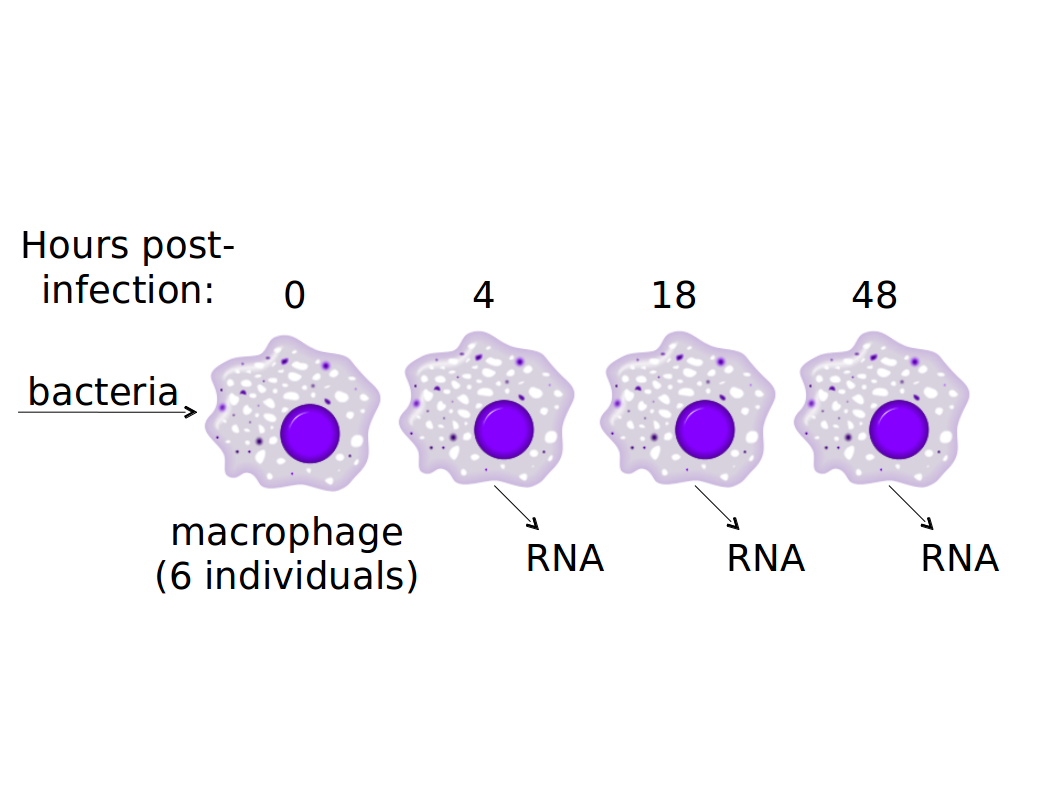
\includegraphics[width=5in]{img/ch02/fig-S01-study-design.png}
\caption[Study design.]{\textbf{Study design.} We infected
  monocyte-derived macrophages isolated from six healthy donors with
  the bacteria described in Table \ref{tab:bacteria}. We isolated RNA
  for sequencing at 4, 18, and 48 hours post-infection.}
\label{fig:study-design}
\end{figure}

\begin{figure}[htbp]
\centering
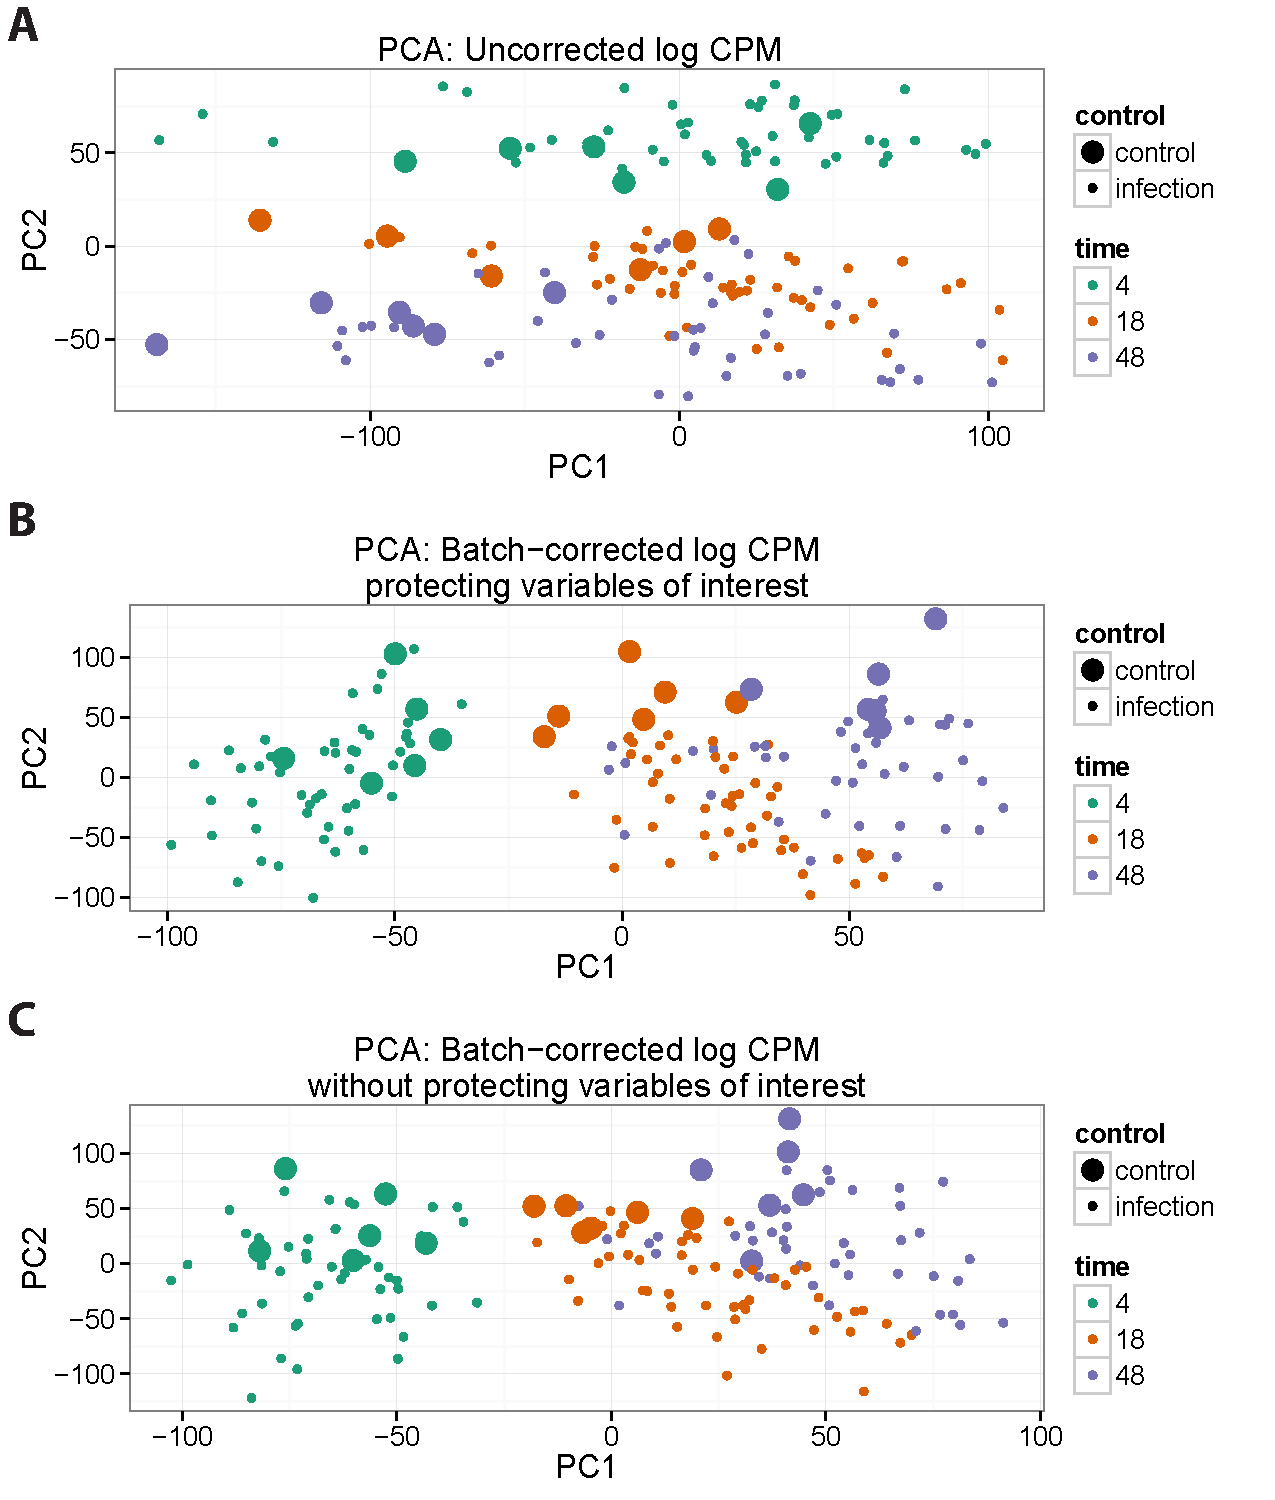
\includegraphics[width=5in]{img/ch02/fig-S02-pca.pdf}
\caption[Principal components analysis (PCA) of uncorrected and
  batch-corrected expression values.]{\textbf{Principal components
    analysis (PCA) of uncorrected and batch-corrected expression
    values.} (A) PCA of the TMM-normalized
  log\textsubscript{2}-transformed counts per million (CPM). Infected
  and control samples are not well separated.  PC2 separates the
  samples by timepoint. (B) PCA of the TMM-normalized
  log\textsubscript{2}-transformed CPM after removing the effects of
  RIN score and processing batch. PC1 separates the samples by
  timepoint. PC2 separates the infected and control samples. (C) PCA
  of the TMM-normalized log\textsubscript{2}-transformed CPM after
  removing the effects of RIN score and processing batch without
  protecting the variables of interest (individual, bacteria,
  timepoint).}
\label{fig:pca}
\end{figure}

\begin{figure}[htbp]
\centering
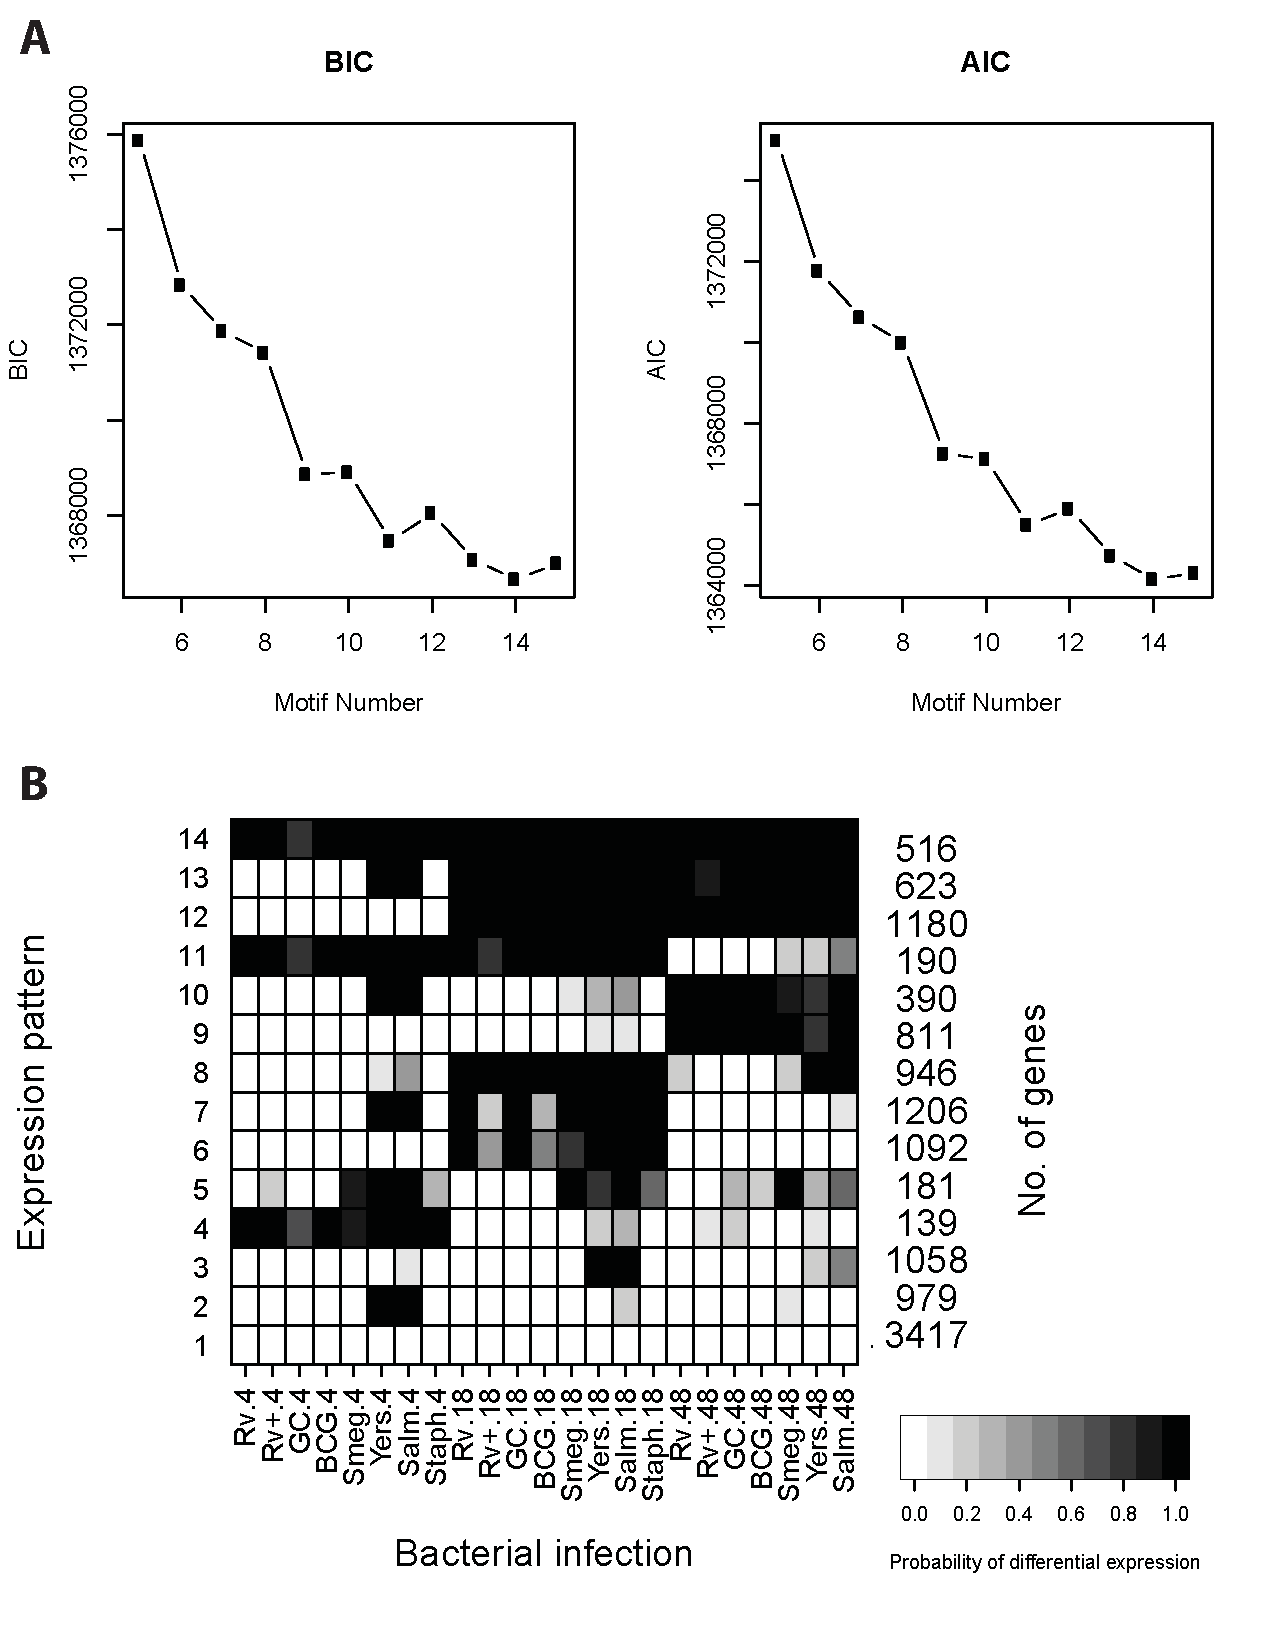
\includegraphics[width=5in]{img/ch02/fig-S03-joint-all-k14.pdf}
\caption[Joint Bayesian analysis with 14 expression
  patterns.]{\textbf{Joint Bayesian analysis with 14 expression
    patterns.} (A) Cormotif \citep{Wei2015} estimates the number of
  expression patterns (i.e.~motifs, using their terminology) to use by
  calculating the Bayesian information criterion (BIC) and the Akaike
  information criterion (AIC). These criteria penalize models for
  additional parameters to avoid overfitting. The model with the
  lowest BIC/AIC is considered the best fit, which in this context is
  the model with 14 expression patterns. (B) Joint analysis with
  Cormotif. The shading of each box represents the posterior
  probability that a gene assigned to the expression pattern (row) is
  differentially expressed in response to infection with a particular
  bacteria (column), with black representing a high posterior
  probability and white a low posterior probability.}
\label{fig:joint-all-k14}
\end{figure}

% Continues caption on next page. Requires package ccaption.
\begin{figure}
  \contcaption{(continued) The expression patterns have the following
    interpretations: ``non-DE'' - Genes that do not respond to
    infection; ``Yers-Salm-4h'' - Genes that respond 4 hours
    post-infection with \emph{Y. pseudotuberculosis} or
    \emph{S. typhimurium}; ``Yers-Salm-18h'' - Genes that respond 18
    hours post-infection with \emph{Y. pseudotuberculosis} or
    \emph{S. typhimurium}; ``4h'' - Genes that respond to 4 hours
    post-infection with any bacteria; ``non-MTB'' - Genes that respond
    at 4, 18, and 48 hours post-infection to bacteria that are not MTB
    or BCG (attenuated \emph{M. bovis}); ``Virulent-18h'' - Genes that
    respond 18 hours post-infection with virulent bacteria;
    ``Virulent-18h+Yers-Salm-4h'' - Genes that respond 18 hours
    post-infection with virulent bacteria and 4 hours post-infection
    with \emph{Y. pseudotuberculosis} or \emph{S. typhimurium};
    ``18h+Yers-Salm-48h'' - Genes that respond 18 hours post-infection
    with any bacteria and 48 hours post-infection with \emph{Y.
      pseudotuberculosis} or \emph{S. typhimurium}; ``48h'' - Genes
    that respond 48 hours post-infection with any bacteria;
    ``48h+Yers-Salm-4h'' - Genes that respond 48 hours post-infection
    with any bacteria and 4 hours post-infection with \emph{Y.
      pseudotuberculosis} or \emph{S. typhimurium}; ``4\&18h'' - Genes
    that respond 4 and 18 hours post-infection with any bacteria;
    ``18\&48h'' - Genes that respond 18 and 48 hours post-infection
    with any bacteria; ``18\&48h+Yers-Salm-4h'' - Genes that respond
    18 and 48 hours post-infection with any bacteria and 4 hours
    post-infection with \emph{Y. pseudotuberculosis} or
    \emph{S. typhimurium}; ``All'' - Genes that respond at 4, 18, and
    48 hours post-infection with any bacteria.}
\end{figure}

\begin{figure}[htbp]
\centering
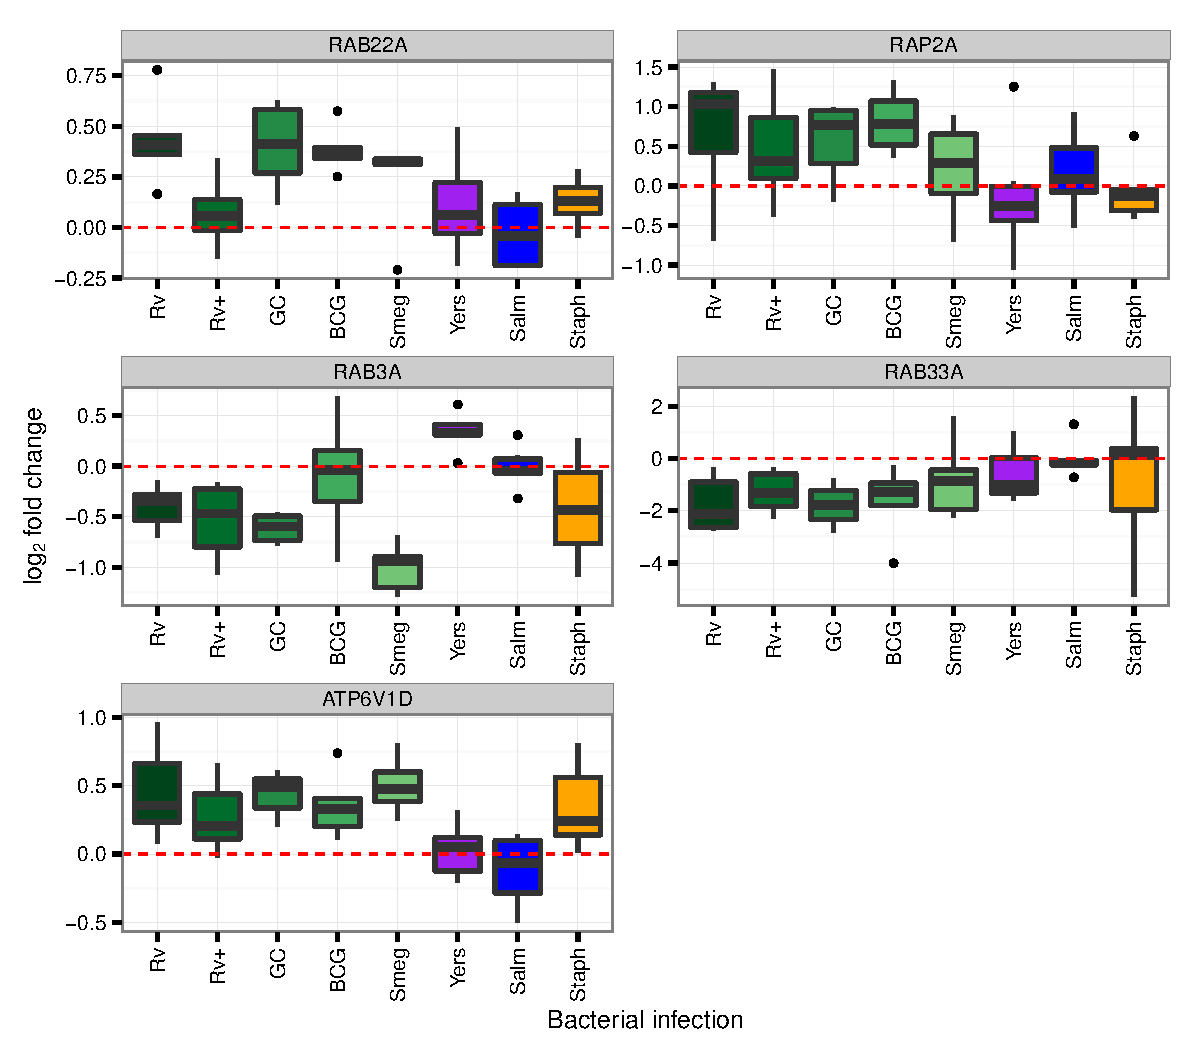
\includegraphics[width=5in]{img/ch02/fig-S04-phago.pdf}
\caption[Expression of genes involved in phagosome
  maturation.]{\textbf{Expression of genes involved in phagosome
    maturation.} \emph{RAB22A}, \emph{RAP2A}, and \emph{ATP6V1D} are
  upregulated in response to infection with mycobacteria at 18 hours;
  whereas, \emph{RAB3A} and \emph{RAB33A} are downregulated (pattern
  ``MTB'' in Figure \ref{fig:joint-18h}).}
\label{fig:phago}
\end{figure}

\begin{figure}[htbp]
\centering
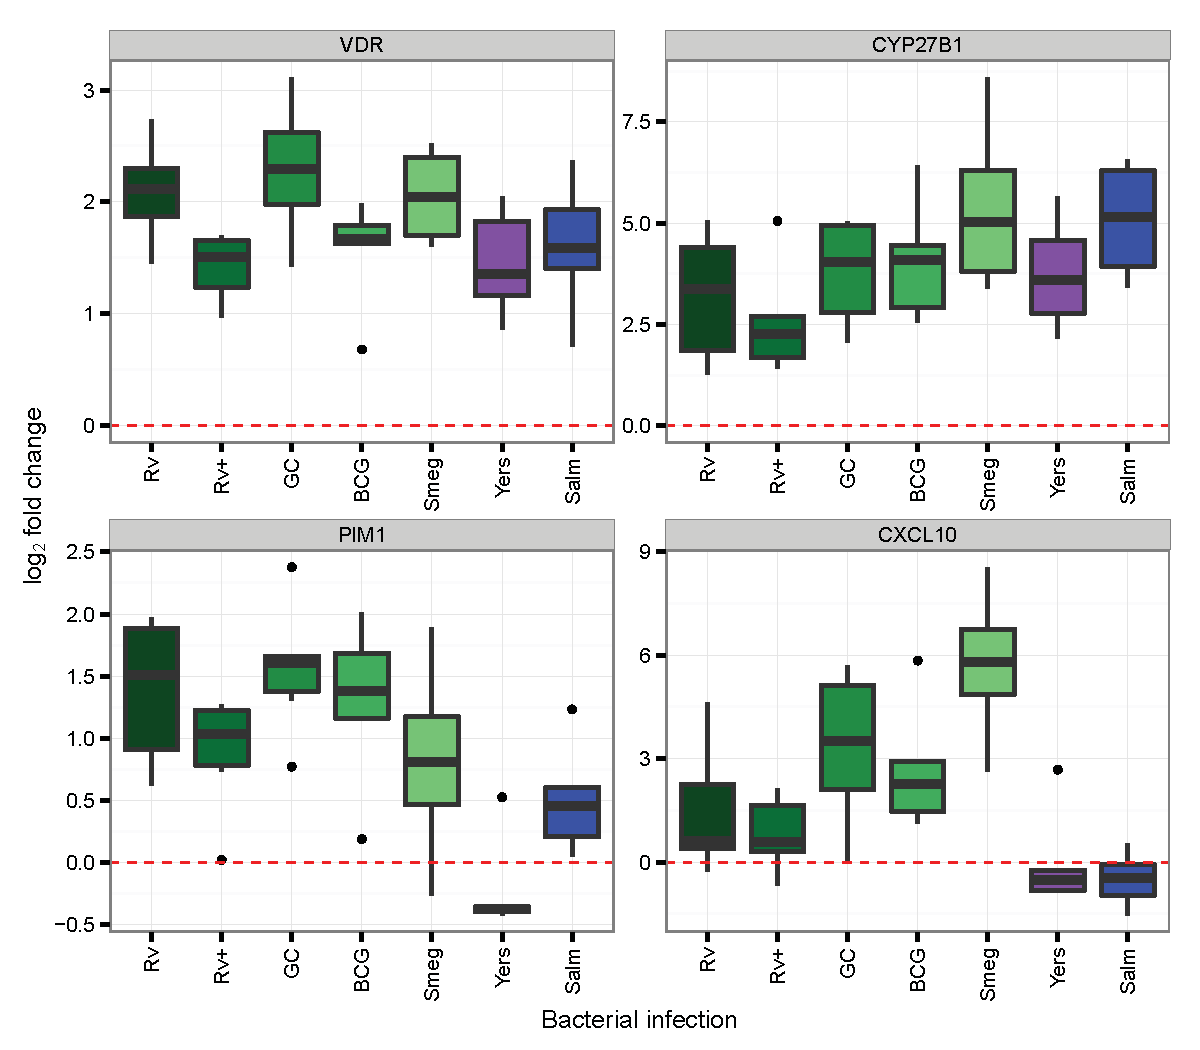
\includegraphics[width=5in]{img/ch02/fig-S05-vitD.pdf}
\caption[Expression of genes involved in vitamin D
  signaling.]{\textbf{Expression of genes involved in vitamin D
    signaling.}  \emph{VDR} and \emph{CYP27B1} are upregulated at 48
  hours post-infection with all bacteria (pattern ``All'' in Figure
  \ref{fig:joint-48h}). \emph{PIM1} and \emph{CXCL10} are upregulated
  at 48 hours post-infection with the mycobacteria (pattern ``MTB'' in
  Figure \ref{fig:joint-48h}).}
\label{fig:vitD}
\end{figure}

\begin{figure}[htbp]
\centering
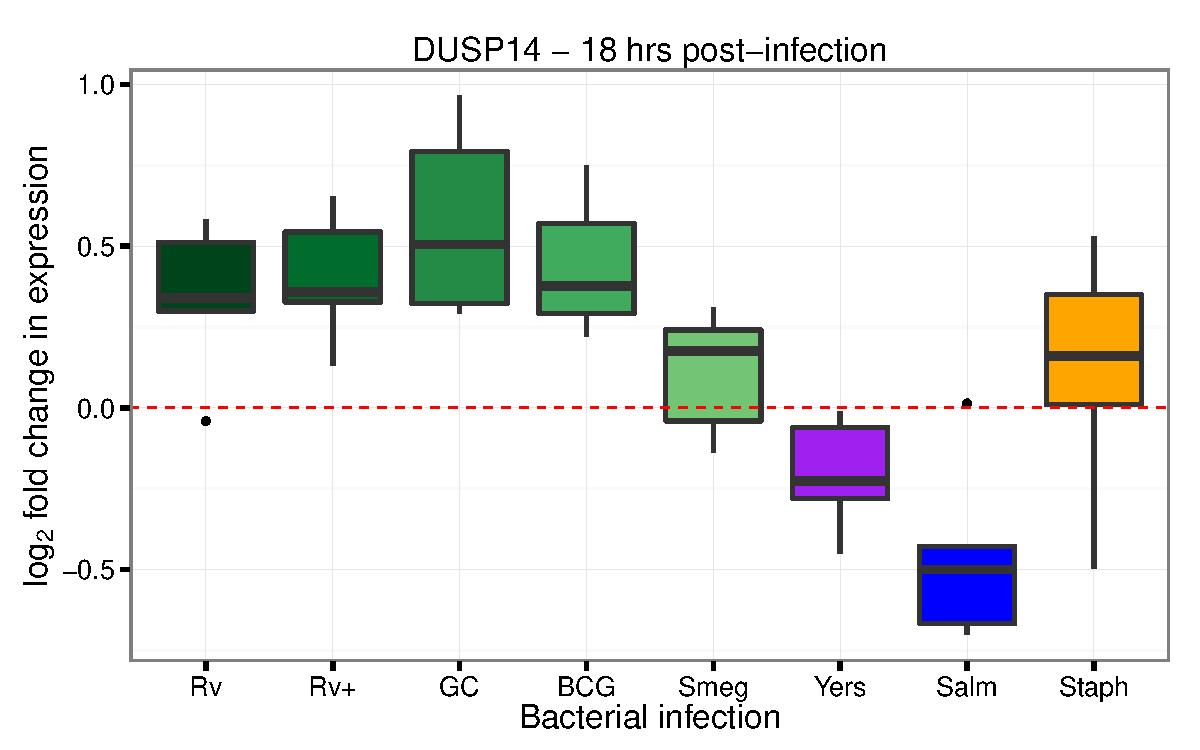
\includegraphics[width=5in]{img/ch02/fig-S06-dusp14.pdf}
\caption[Expression of \emph{DUSP14} at 18 hours
  post-infection.]{\textbf{Expression of \emph{DUSP14} at 18 hours
    post-infection.} \emph{DUSP14} is an example of an interesting
  gene not identified with our approach. At 18 hours, it is
  upregulated after infection with MTB H37Rv (q-value: 16\%), MTB
  GC1237 (q-value: 3\%), and BCG (q-value: 9\%) (the change in
  heat-inactivated MTB H37Rv had a q-value of 26\%); and downregulated
  post-infection with \emph{S. typhimurium} (q-value: 9\%).  Because
  it did not fit well into one of the main patterns of gene expression
  identified at 18 hours post-infection, it was classified as the
  ``non-DE'' pattern.}
\label{fig:dusp14}
\end{figure}

\begin{figure}[htbp]
\centering
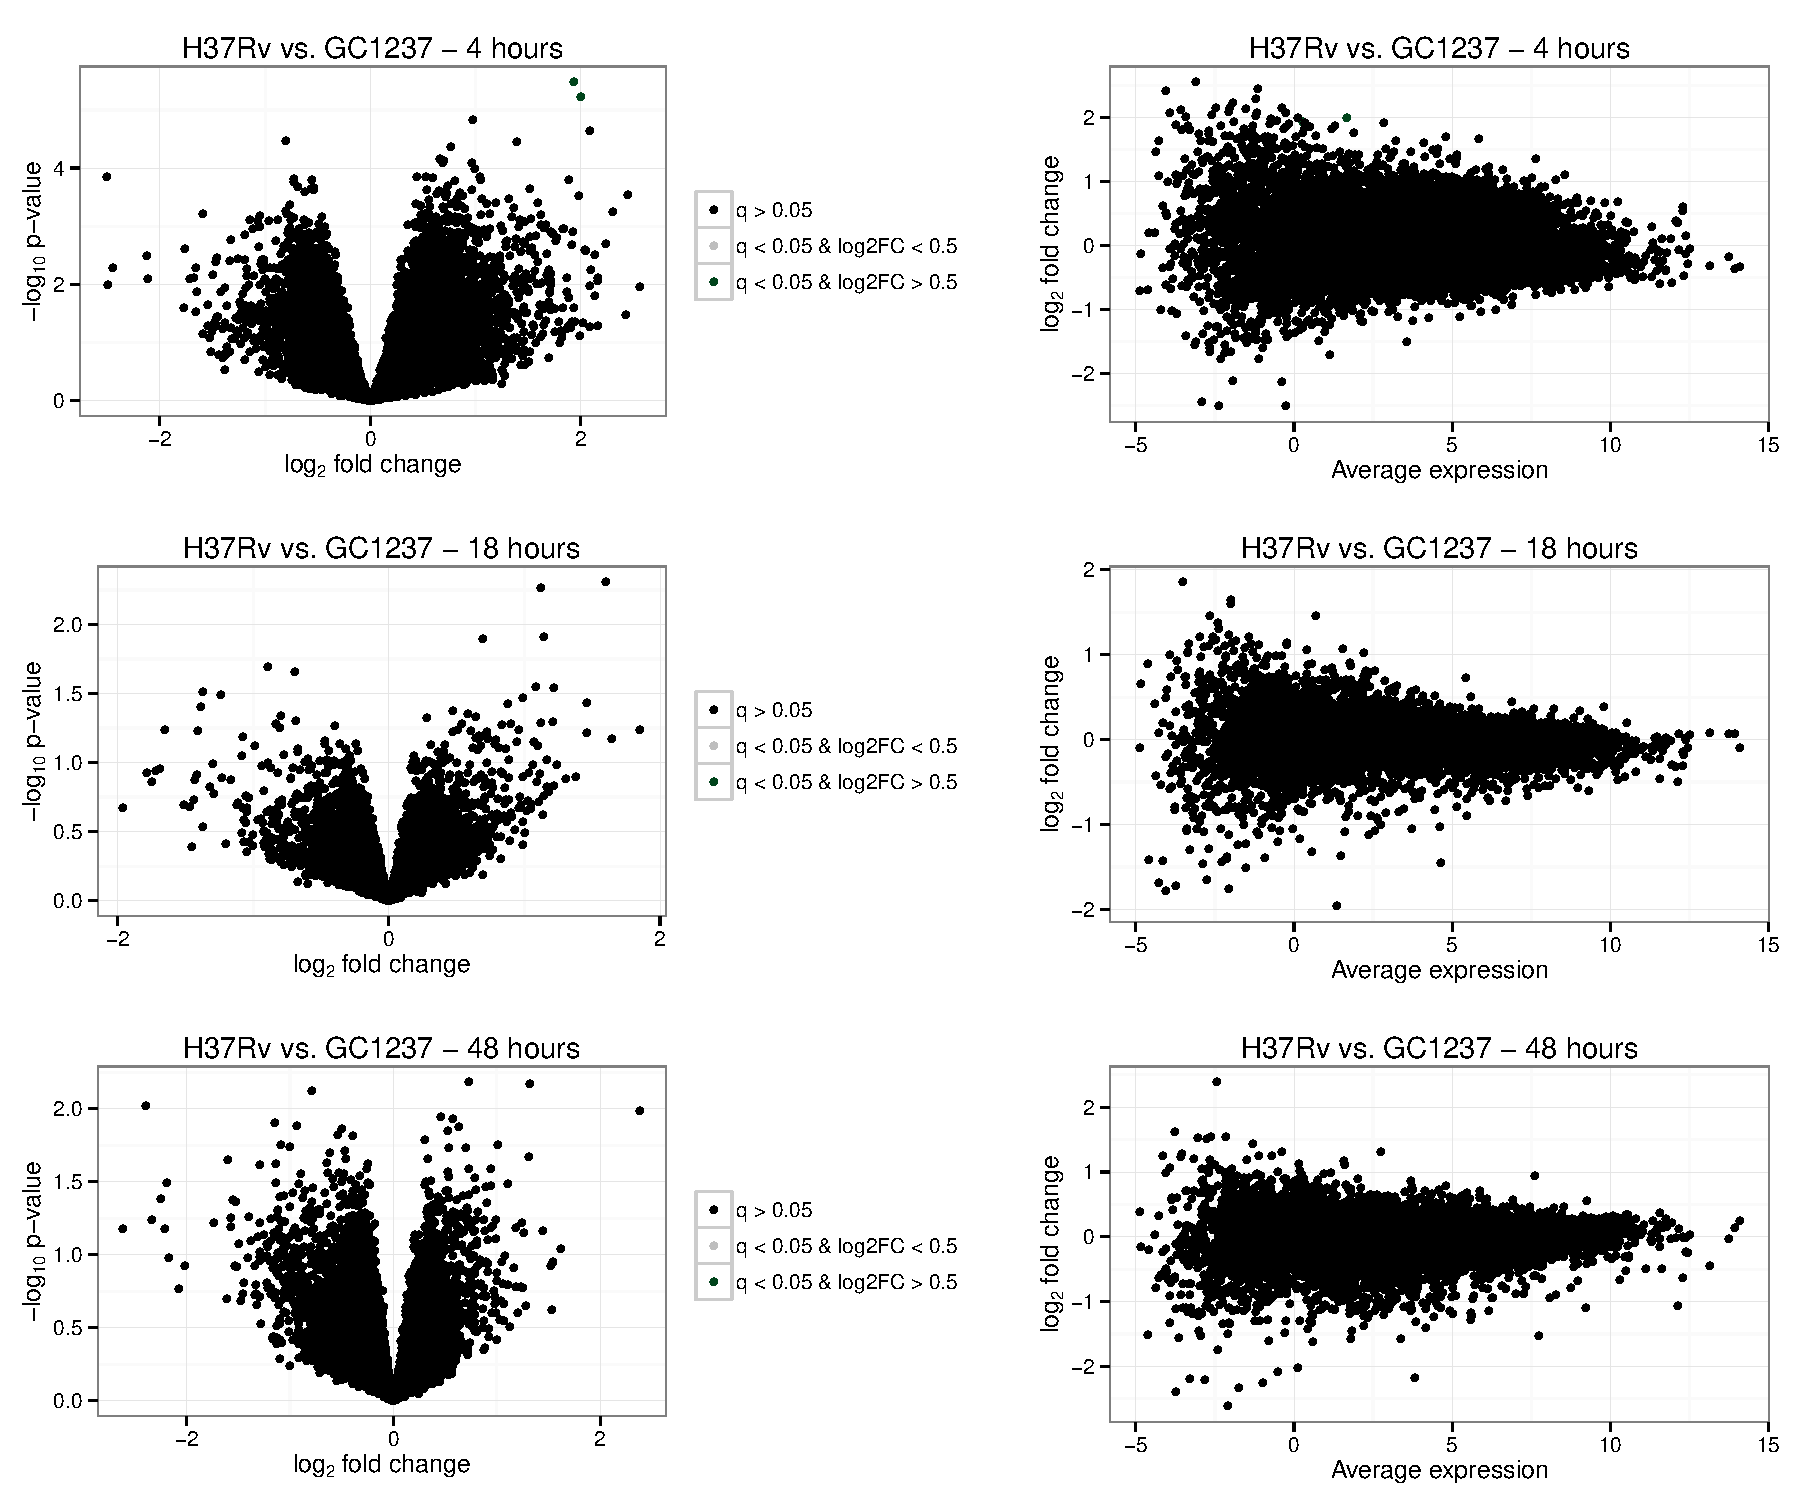
\includegraphics[width=5in]{img/ch02/fig-S07-Rv-v-GC.pdf}
\caption[Little difference in transcriptional response to infections
  with different MTB strains.]{\textbf{Little difference in
    transcriptional response to infections with different MTB
    strains.} Few statistically significant differences were
  identified when explicitly testing gene expression levels
  post-infection with MTB H37Rv and MTB GC1237 at 4, 18, or 48 hours
  post-infection (top, middle, and bottom panels, respectively). The
  volcano plots (left) display the -log\textsubscript{10} transformed
  p-value versus the log\textsubscript{2} fold change in expression
  level. The MA plots (right) display the log\textsubscript{2} fold
  change in expression level versus the average expression level. Most
  of the genes are labeled black indicating that their FDR value is
  greater than 5\%. Two genes (labeled green) at 4 hours
  post-infection had a q-value \textless{} 0.05 and
  log\textsubscript{2} fold change greater than 0.5 (see Supplementary
  Table \ref{tab:s8}).}
\label{fig:Rv-v-GC}
\end{figure}

\begin{figure}[htbp]
\centering
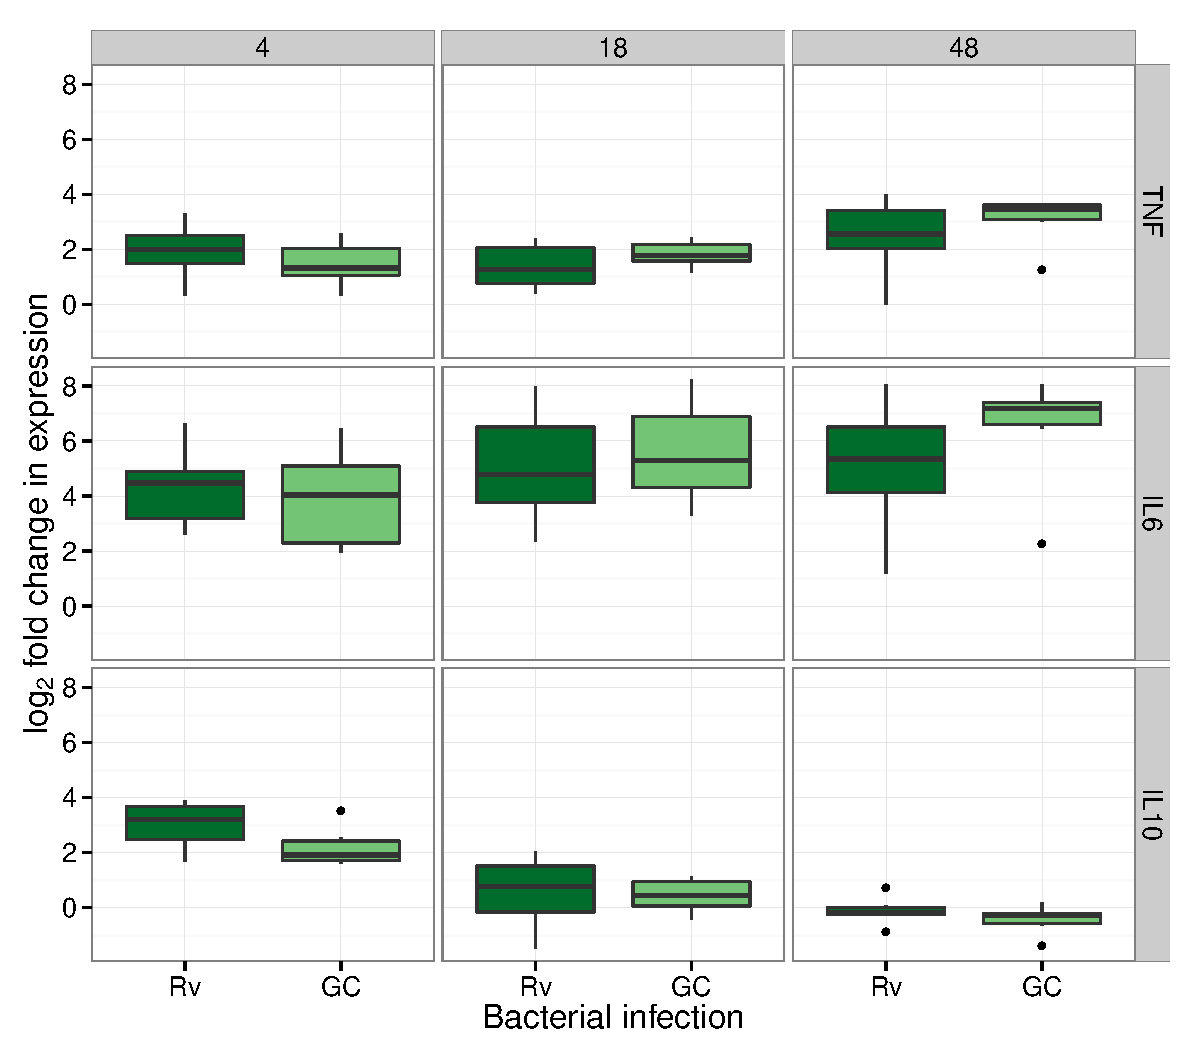
\includegraphics[width=5in]{img/ch02/fig-S08-ex-cytokines.pdf}
\caption[Response of example cytokines to infection with different MTB
  strains.]{\textbf{Response of example cytokines to infection with
    different MTB strains.} The log\textsubscript{2} fold change in
  expression of the pro-inflammatory cytokines \emph{TNF} and
  \emph{IL6} and the anti-inflammatory cytokine \emph{IL10} is similar
  post-infection with MTB H37Rv or MTB GC1237. \emph{TNF} and
  \emph{IL6} are upregulated at all three timepoints; whereas,
  \emph{IL10} is upregulated only at 4 hours post-infection.}
\label{fig:ex-cytokines}
\end{figure}

\begin{figure}[htbp]
\centering
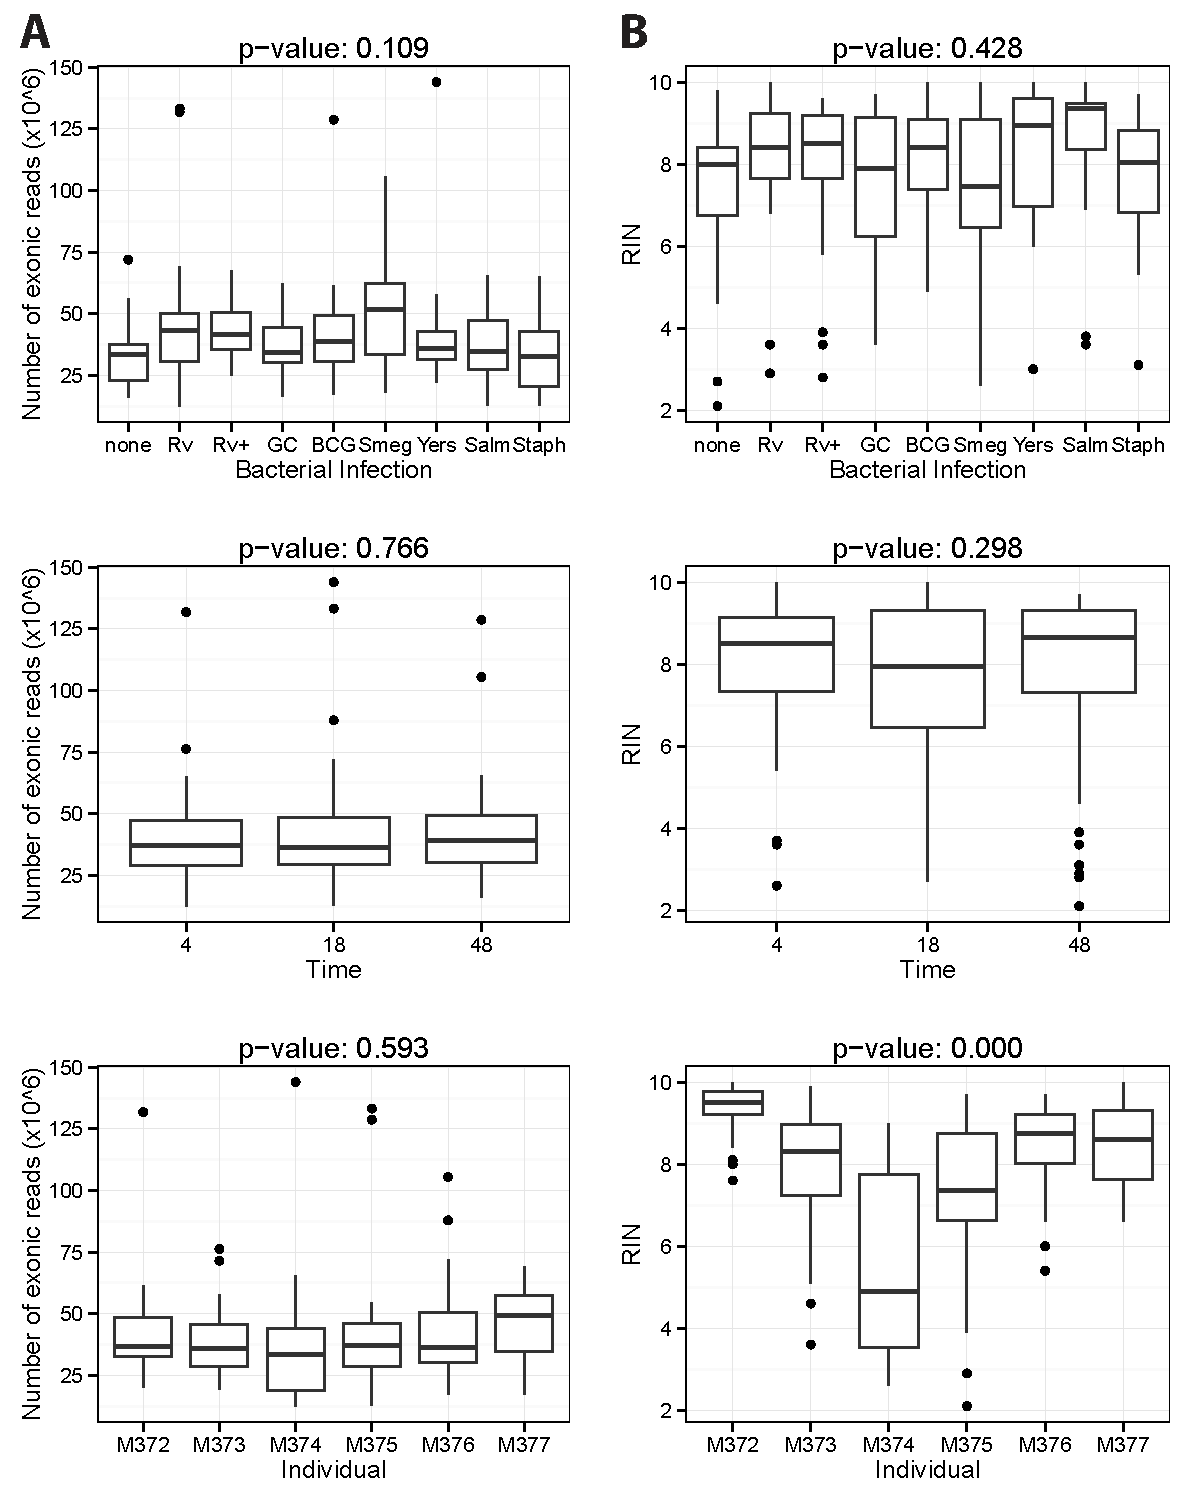
\includegraphics[width=5in]{img/ch02/fig-S09-rin-and-reads.pdf}
\caption[Distribution of the number of exonic reads and RNA quality
  scores (RIN) across variables of interest.]{\textbf{Distribution of
    the number of exonic reads and RNA quality scores (RIN) across
    variables of interest.} (A) The number of exonic reads is evenly
  distributed across the bacterial infections, timepoints, and
  individuals. (B) The RIN scores are evenly distributed across the
  bacterial infections and timepoints; however, the RIN does vary
  between the individuals.  The p-values are from an F-test.}
\label{fig:rin-and-reads}
\end{figure}

\begin{figure}[htbp]
\centering
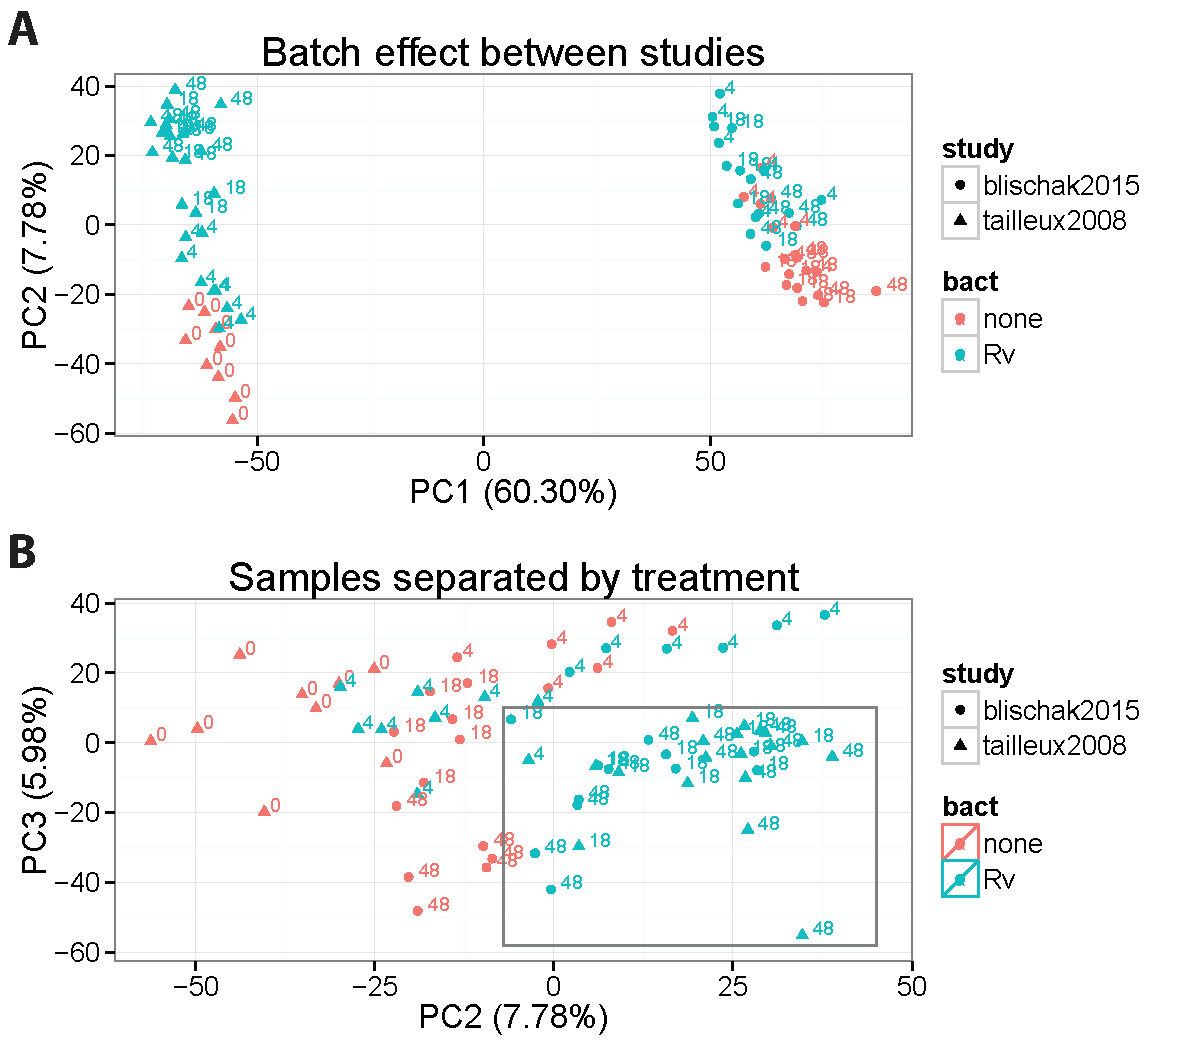
\includegraphics[width=5in]{img/ch02/fig-S10-tailleux2008.pdf}
\caption[Comparison to Tailleux et al., 2008.]{\textbf{Comparison to
    Tailleux et al., 2008.} We compared our RNA-seq data to the
  microarray data of Tailleux et al., 2008 \citep{Tailleux2008} to
  confirm a consistent signature of infection.  From our experiment,
  we used the batch-corrected TMM-normalized
  log\textsubscript{2}-transformed counts per million (CPM) from the
  MTB H37Rv infected macrophages at 4, 18, and 48 hours post-infection
  and their time-matched controls. From their experiment, we used the
  log\textsubscript{2}-transformed quantile-normalized data from the
  MTB H37Rv infected macrophages at 4, 18, and 48 hours post-infection
  as well as the zero timepoint non-infection control. In addition to
  the difference in technology, the macrophages were isolated via
  positive selection in our study and negative selection in
  theirs. Despite these differences, we still observe a common
  transcriptional signature of infection when performing principal
  components analysis (PCA). (A) PC1 is the expected batch effect
  between the two experiments. (B) Plotting PC2 versus PC3, the
  infected samples at 18 and 48 hours (when there is a strong
  transcriptional response; see Figure 1A) from the two different
  studies cluster together. The quantile-normalized data from Tailleux
  et al., 2008 \citep{Tailleux2008} is available at
  https://bitbucket.org/jdblischak/tb-data.}
\label{fig:tailleux2008}
\end{figure}
